\section{Istruzione utilizzo utente amministratore}

La seguente sezione fornirà indicazioni utili per il corretto utilizzo del software nel caso l'utente interessato sia l'amministratore.

\subsection{Login}
Il primo passo da effettuare è l'inserimento del proprio codice identificativo e password all'interno dei campi visualizzati nella pagina di login. Dopo aver premuto il pulsante di conferma, si sarà indirizzati alla pagina dedicata alle funzionalità di amministratore. Nel caso le credenziali inserite non risultino corrette, sarà visualizzato un messaggio d'errore e sarà quindi necessario inserire di nuovo i dati.
\begin{figure}[H]
    \centering
    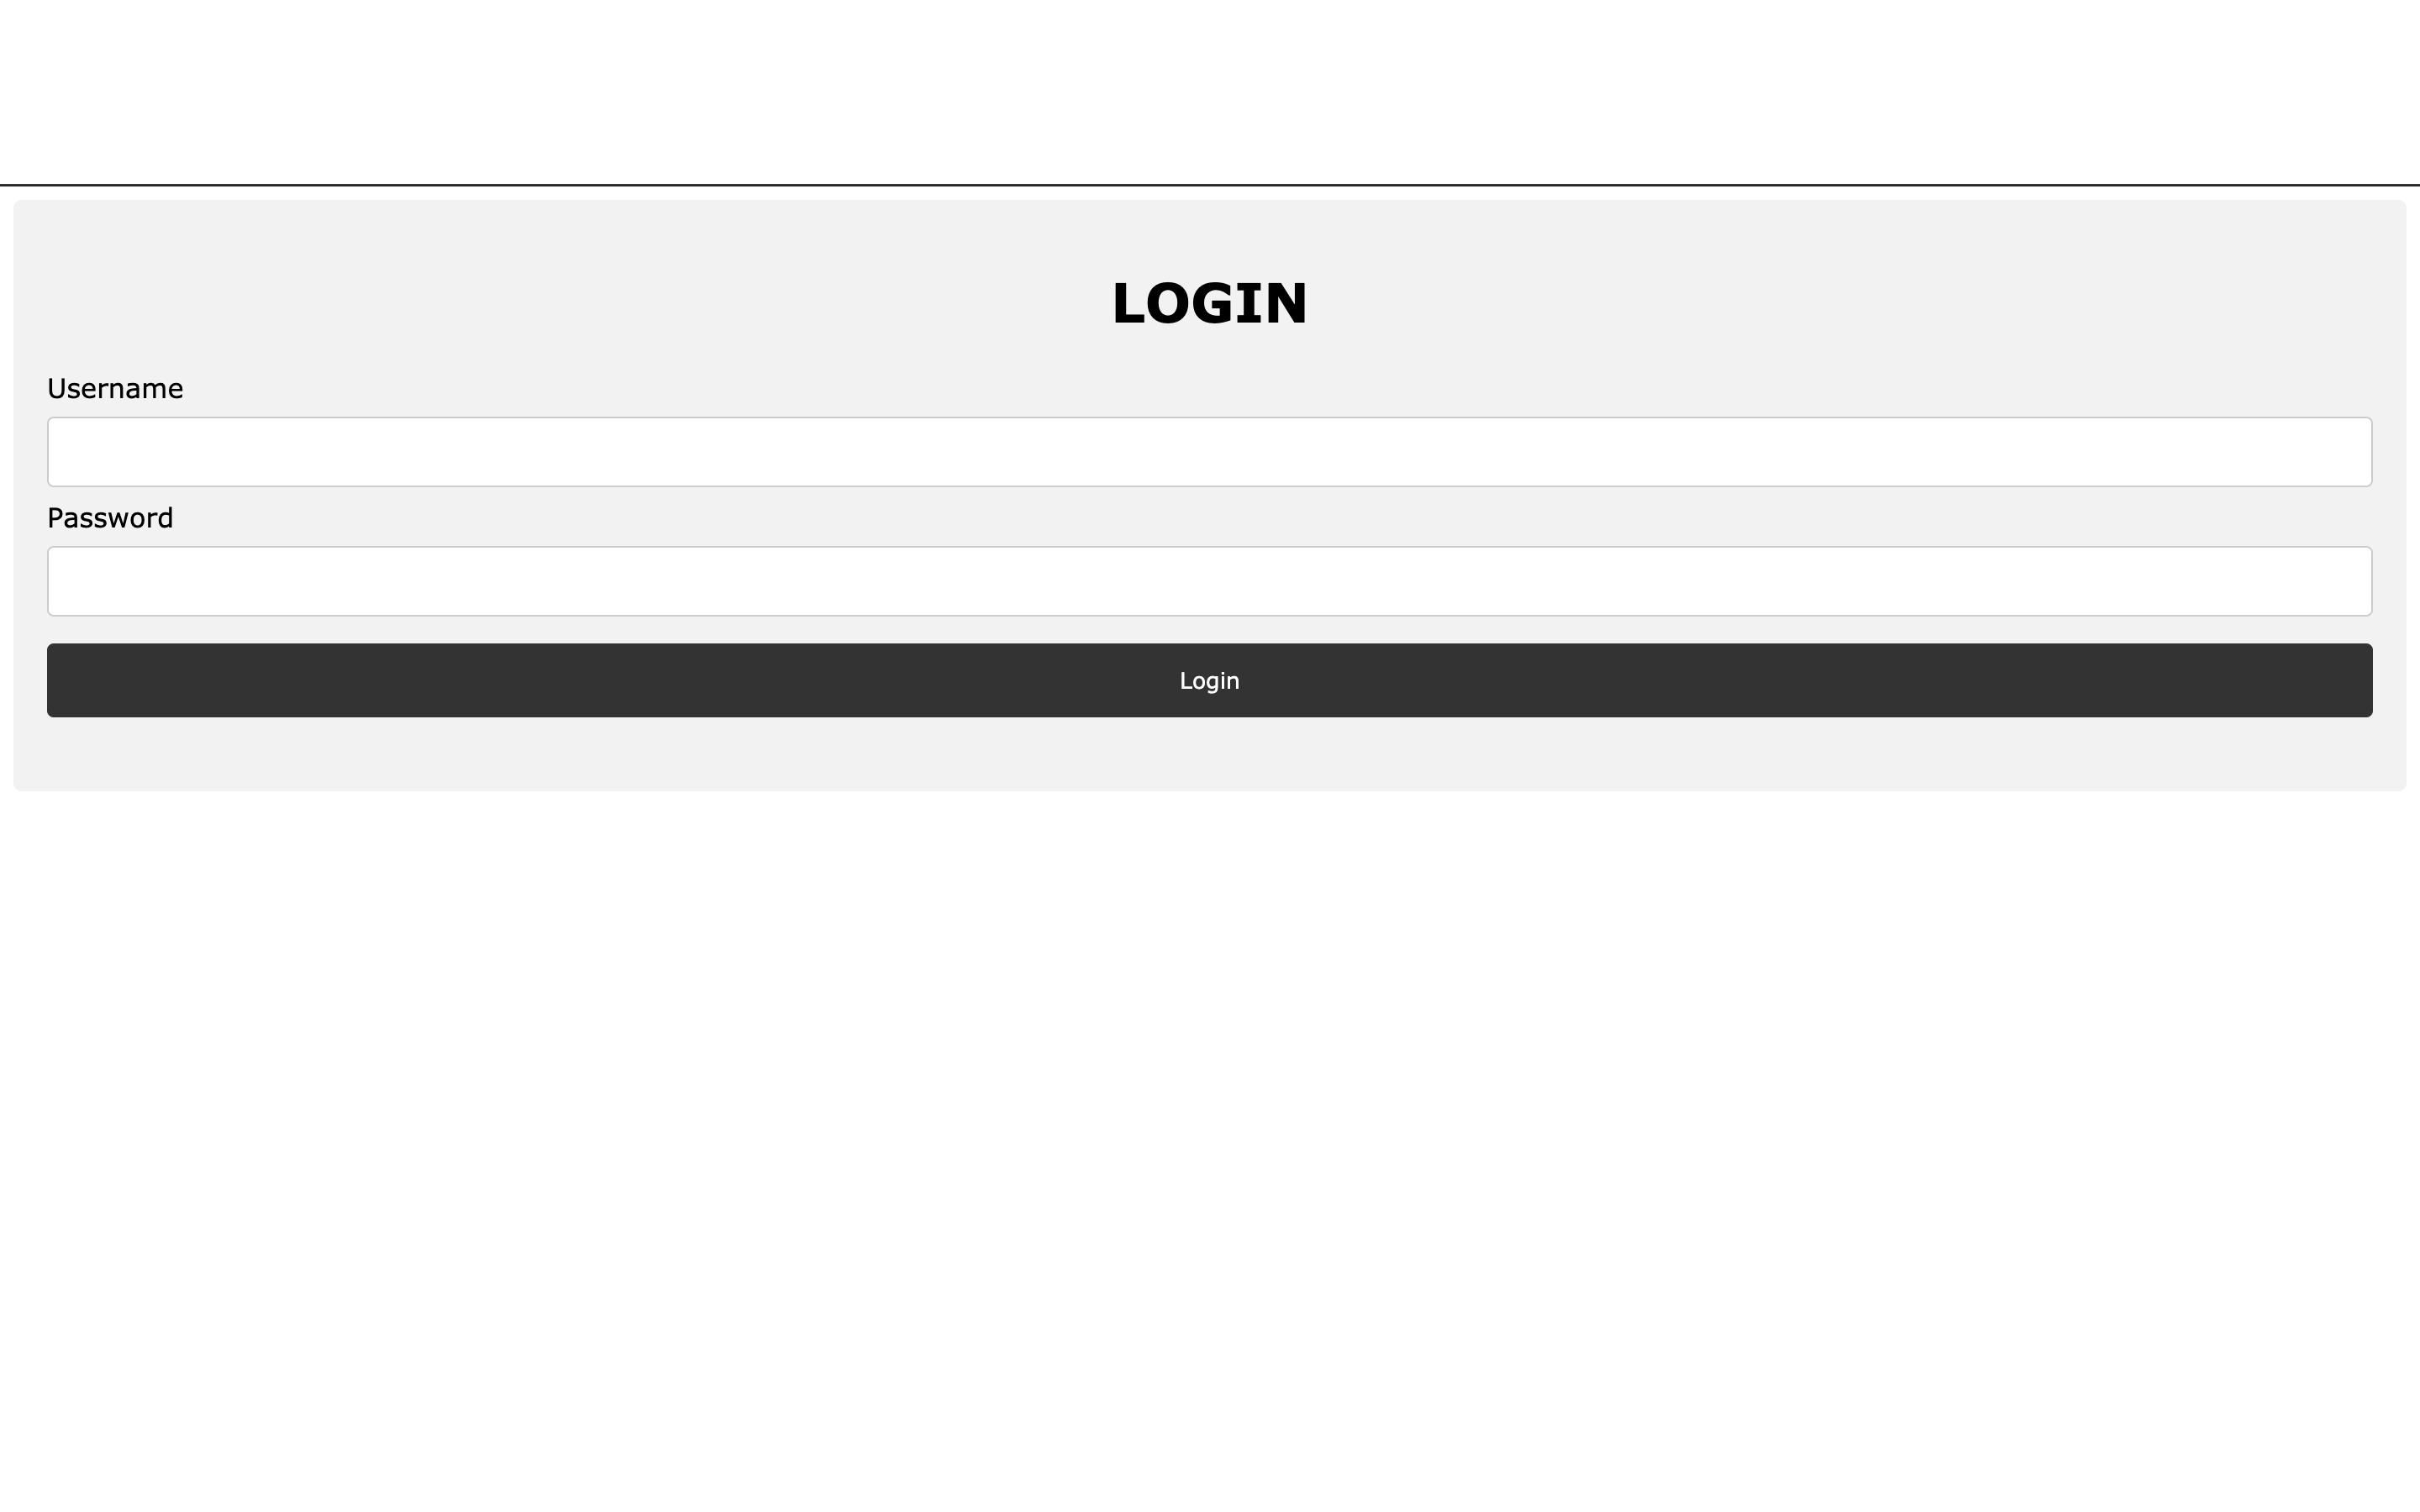
\includegraphics[scale=0.12]{res/images/login.png}
    \caption{Login}
\end{figure}
\subsection{Visualizzazione situazione in real time del magazzino}
\begin{itemize}
    \item Dopo l'autenticazione, tramite il menù selezionare il pulsante "Mappa";
    \item viene visualizzata la planimetria del magazzino con la relativa legenda e la rappresentazione dei muletti che si spostano;
    \item la tabella a destra rappresentano le liste di task con i relativi muletti che le stanno soddisfando.
    
\end{itemize}

\begin{figure}[H]
    \centering
    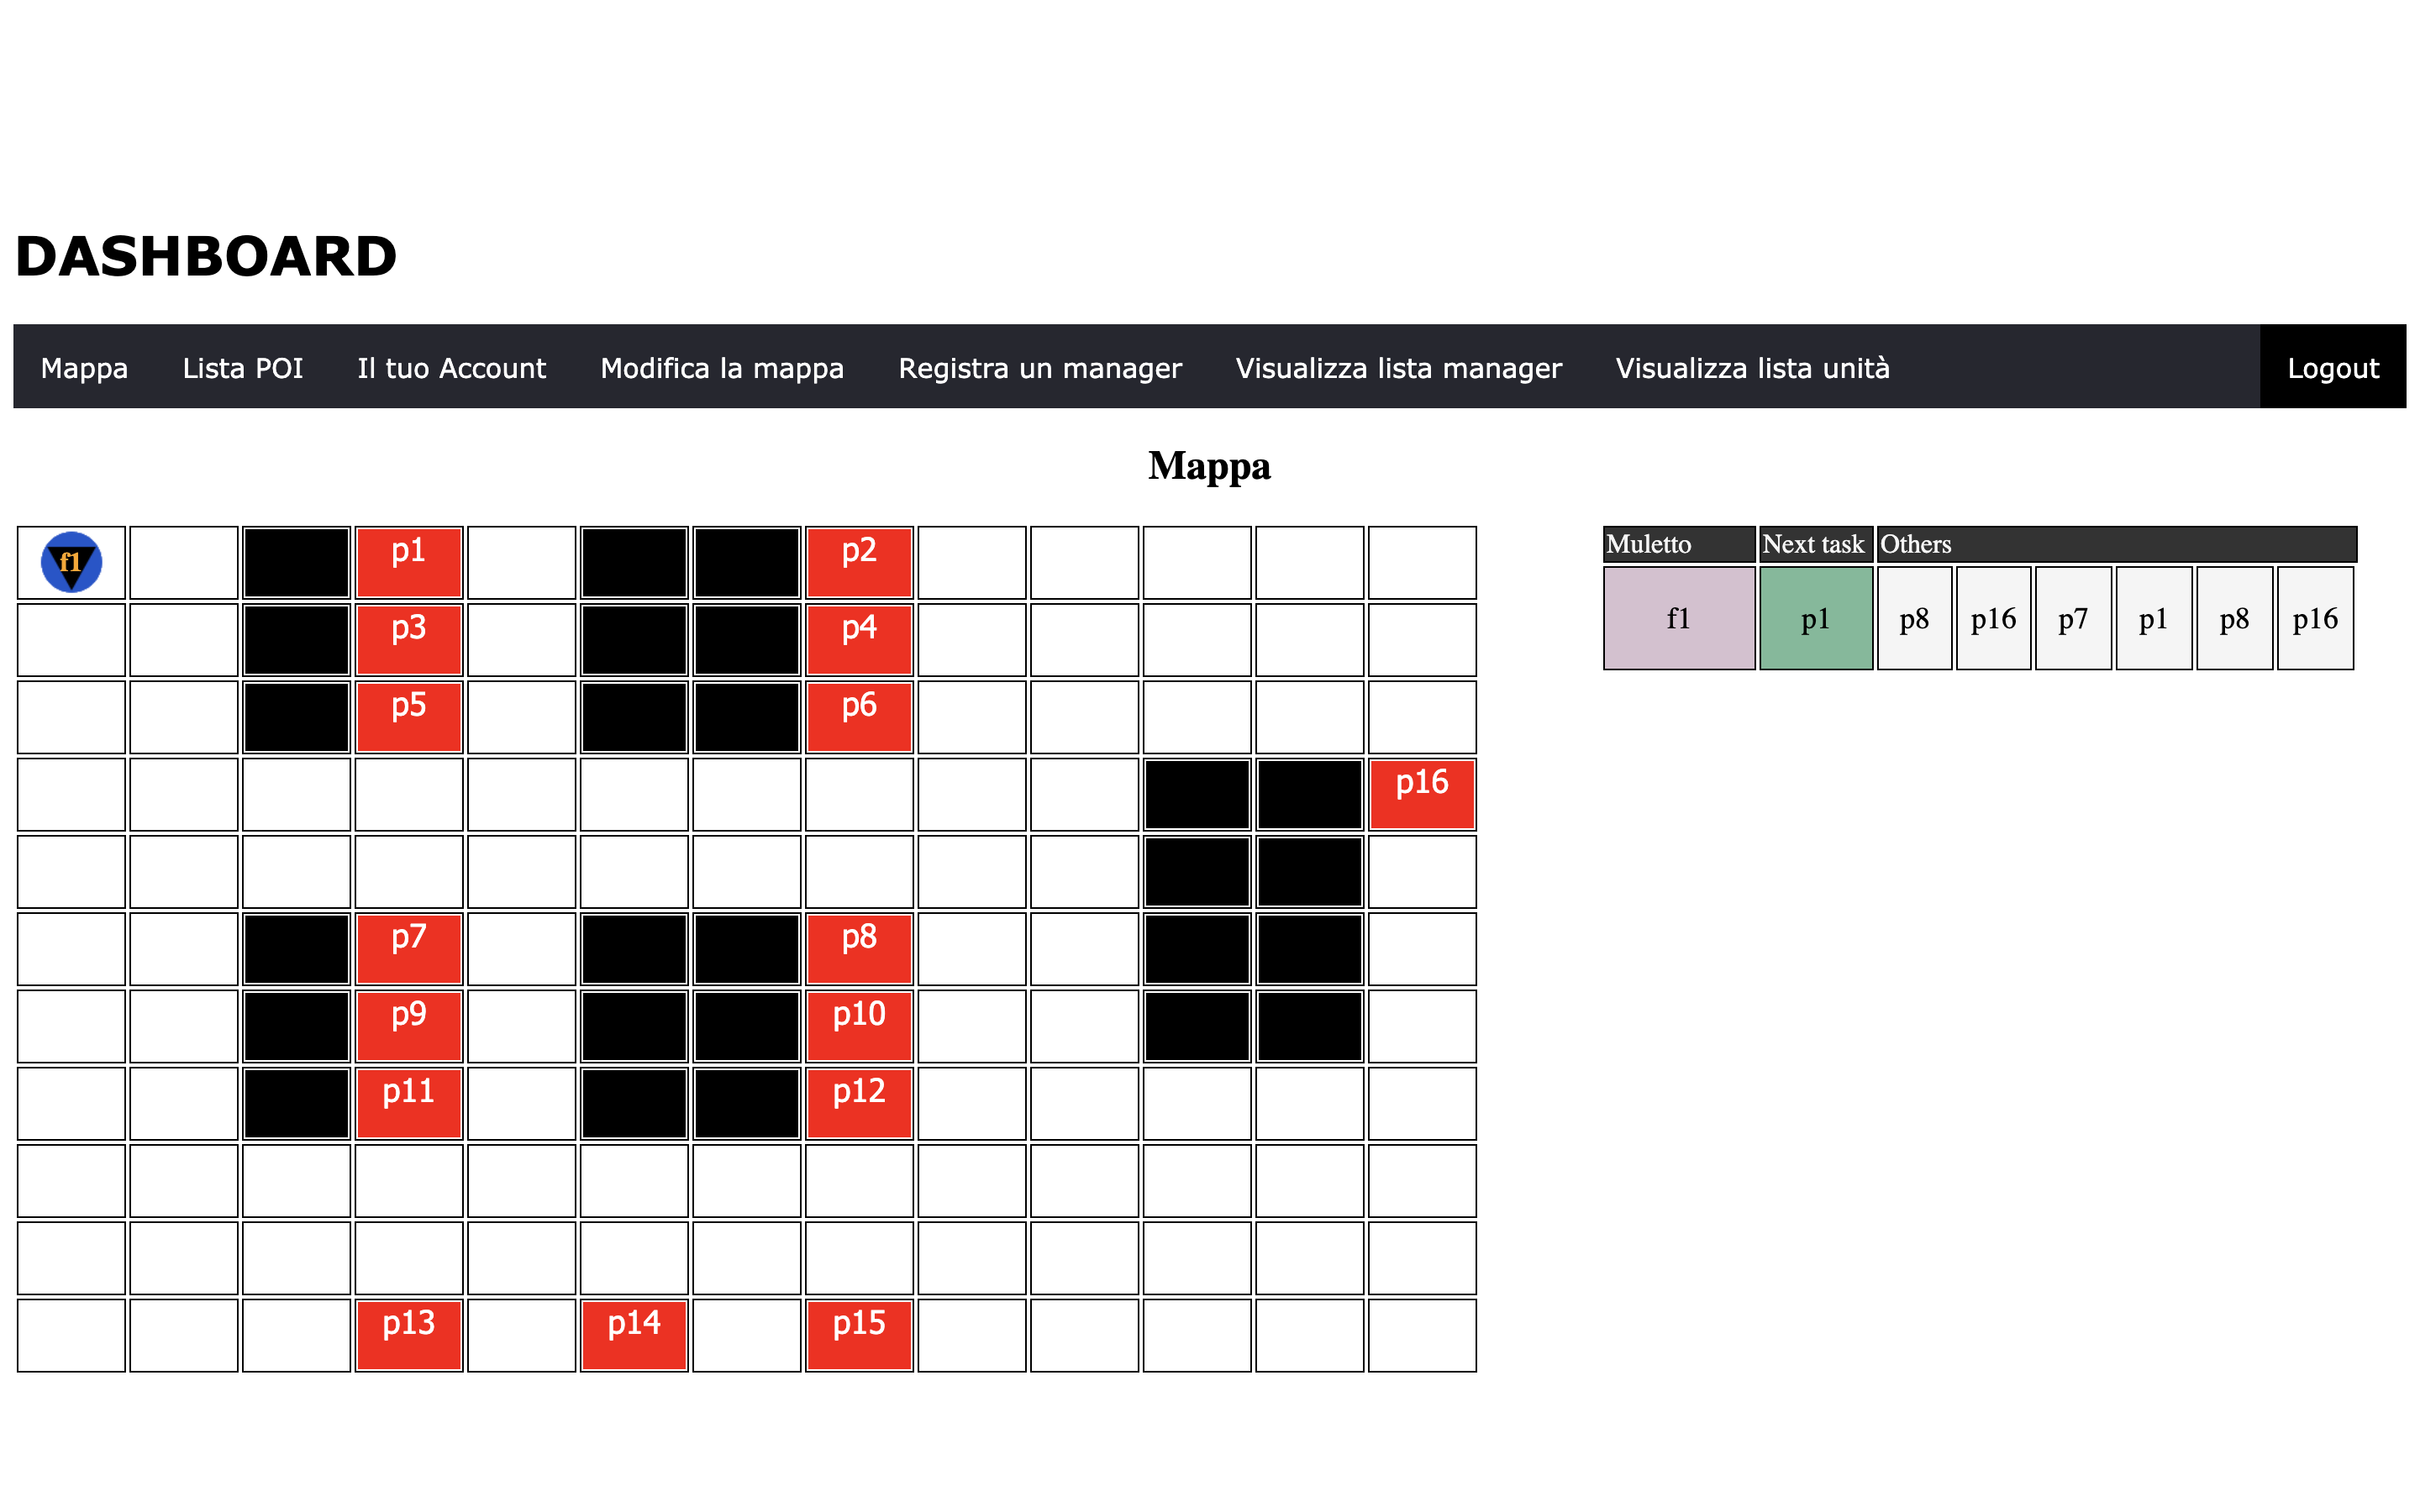
\includegraphics[scale=0.12]{res/images/map_user.png}
    \caption{Schermata visualizzazione in real time del magazzino}
\end{figure}

\subsection{Visualizzazione lista completa punti di interesse}
\begin{itemize}
    \item Dopo l'autenticazione, tramite il menù selezionare il pulsante "Lista POI";
    \item si viene indirizzati alla pagina con l'elenco di tutti i punti di interesse presenti nel magazzino.

\end{itemize}

\begin{figure}[H]
    \centering
    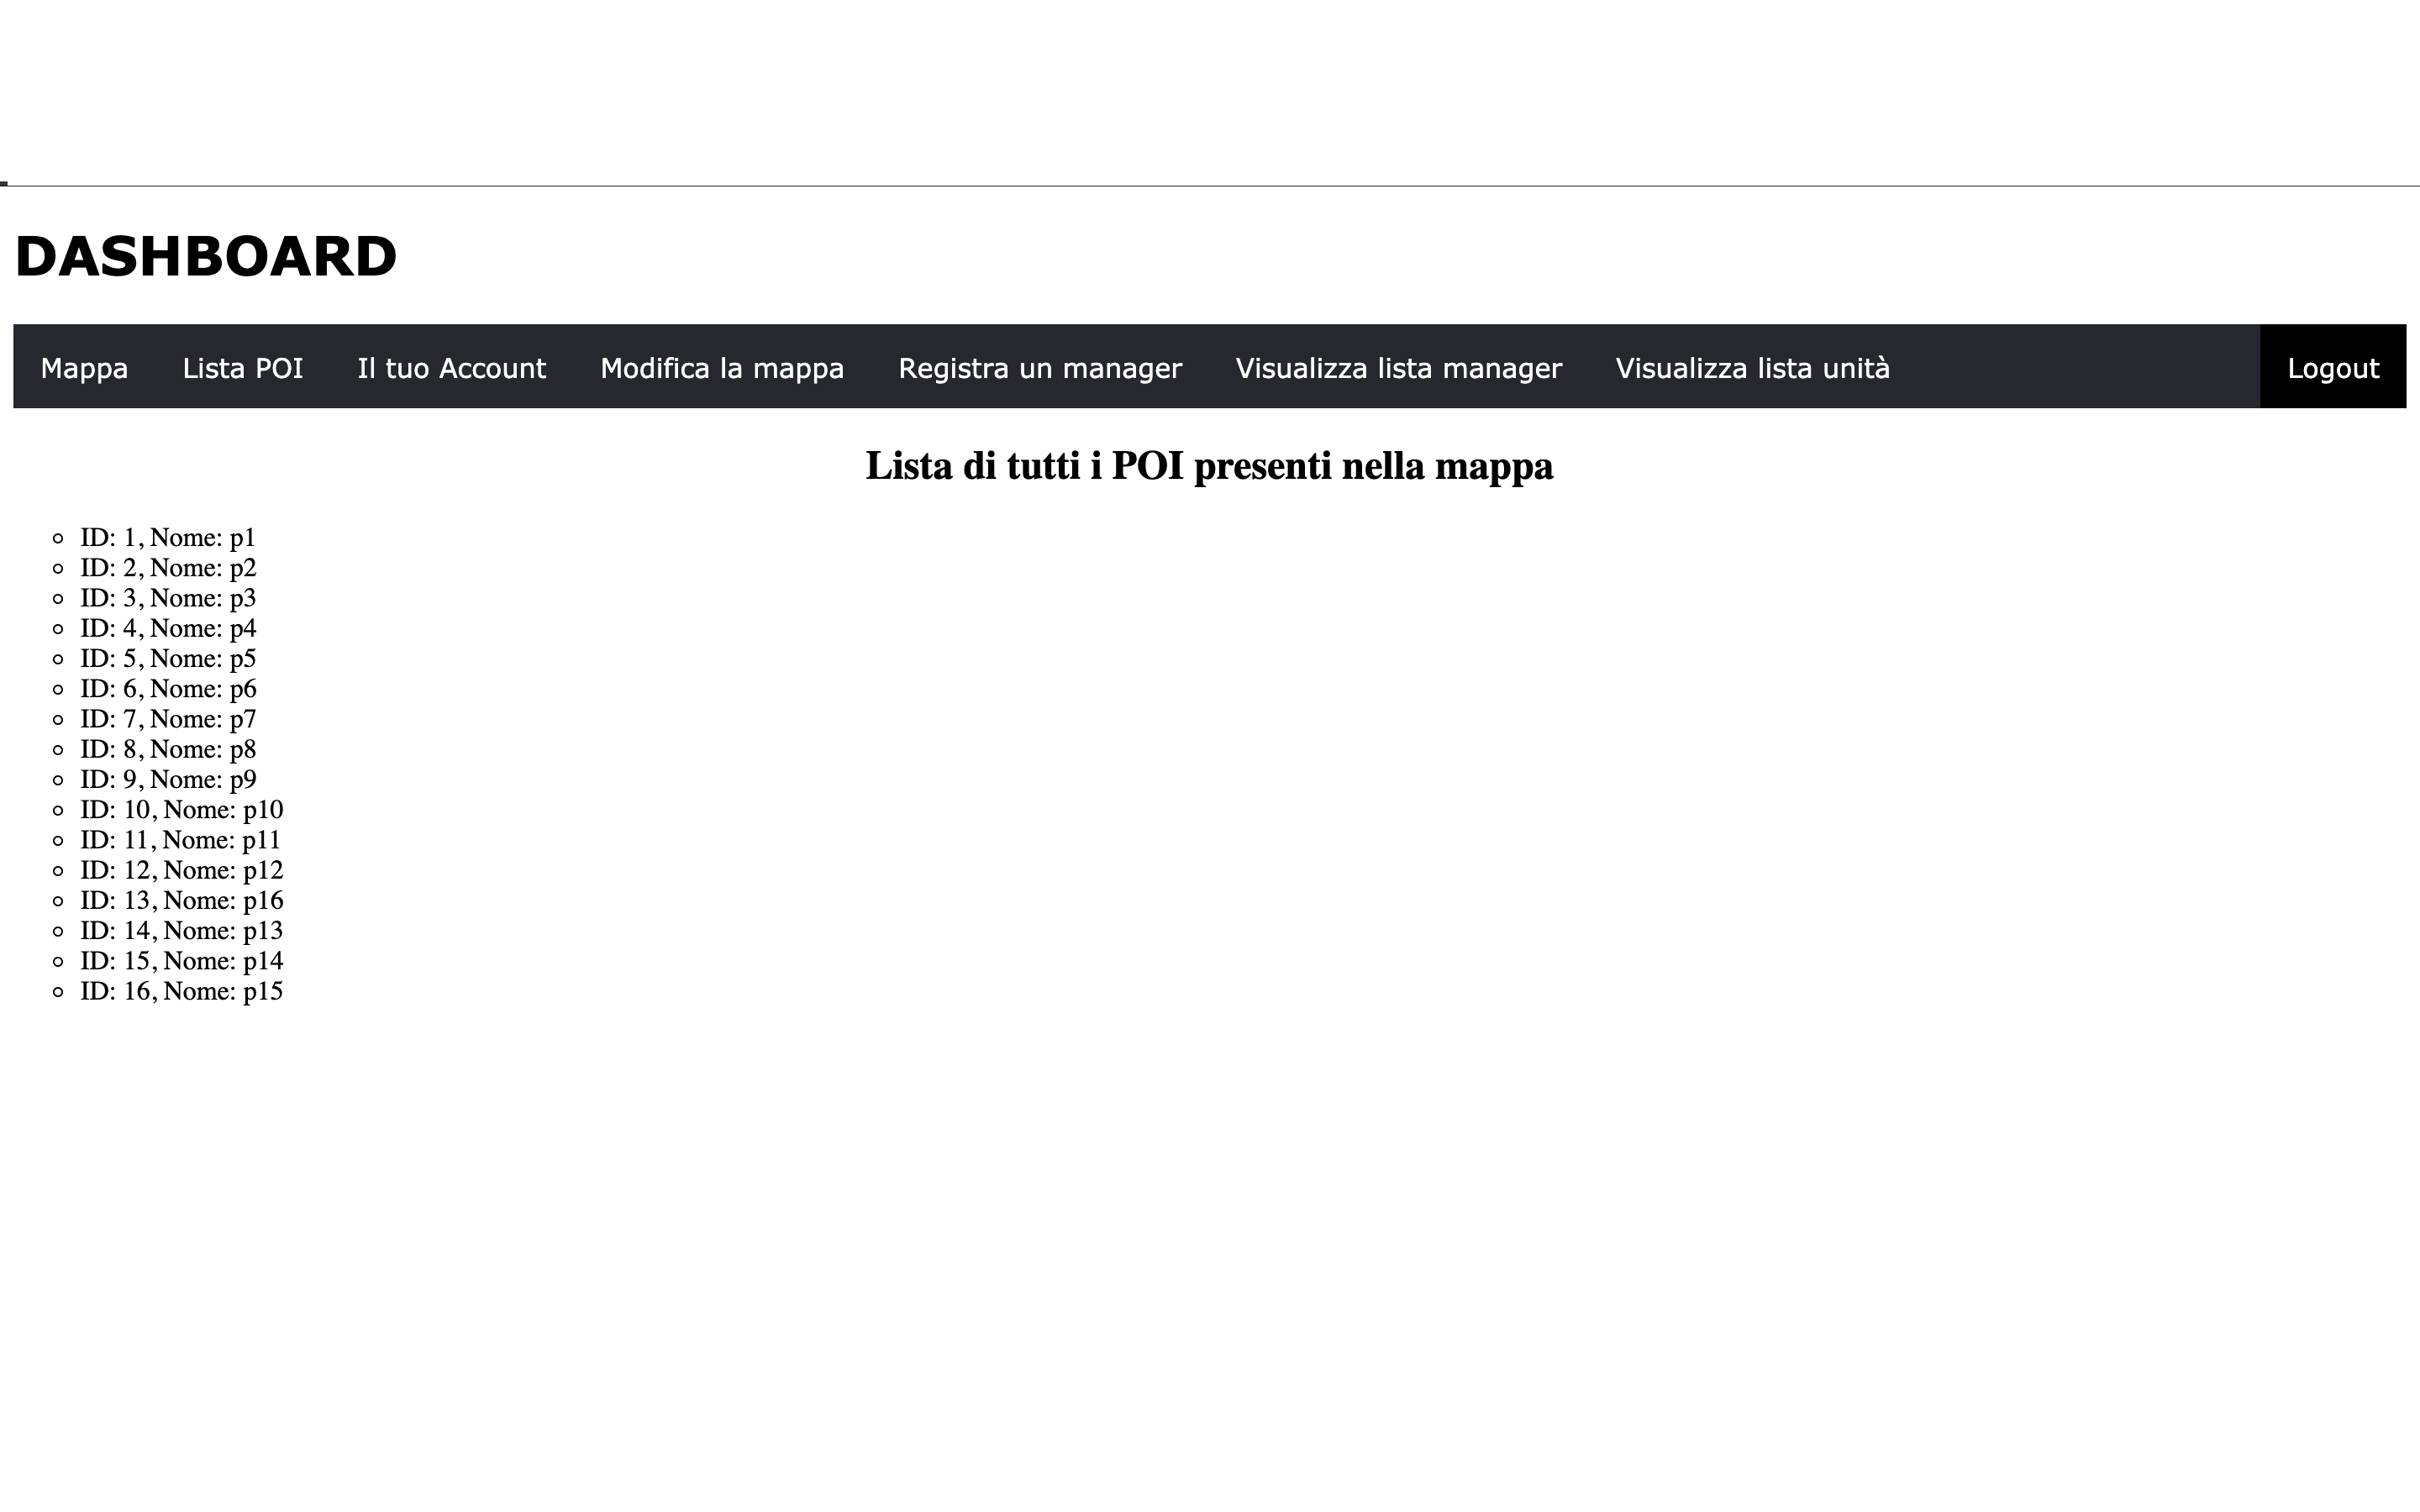
\includegraphics[scale=0.12]{res/images/listpoi_user.png}
    \caption{Schermata guida automatica dell'unità}
\end{figure}

\subsection{Visualizzazione dati del proprio profilo e modifica}
\begin{itemize}
    \item Dopo l'autenticazione, tramite il menù selezionare il pulsante "Il tuo account";
    \item si viene indirizzati alla pagina con i propri dati utente: Name, Surname, Password;
    \item se si desidera modificare alcuni campi, è necessario scrivere nell'apposito form i nuovi dati e premere il pulsante "Salva Modifiche". Se si intende cambiare la Password, l'inserimento nei due campi deve coincidere.
\end{itemize}
\begin{figure}[H]
    \centering
    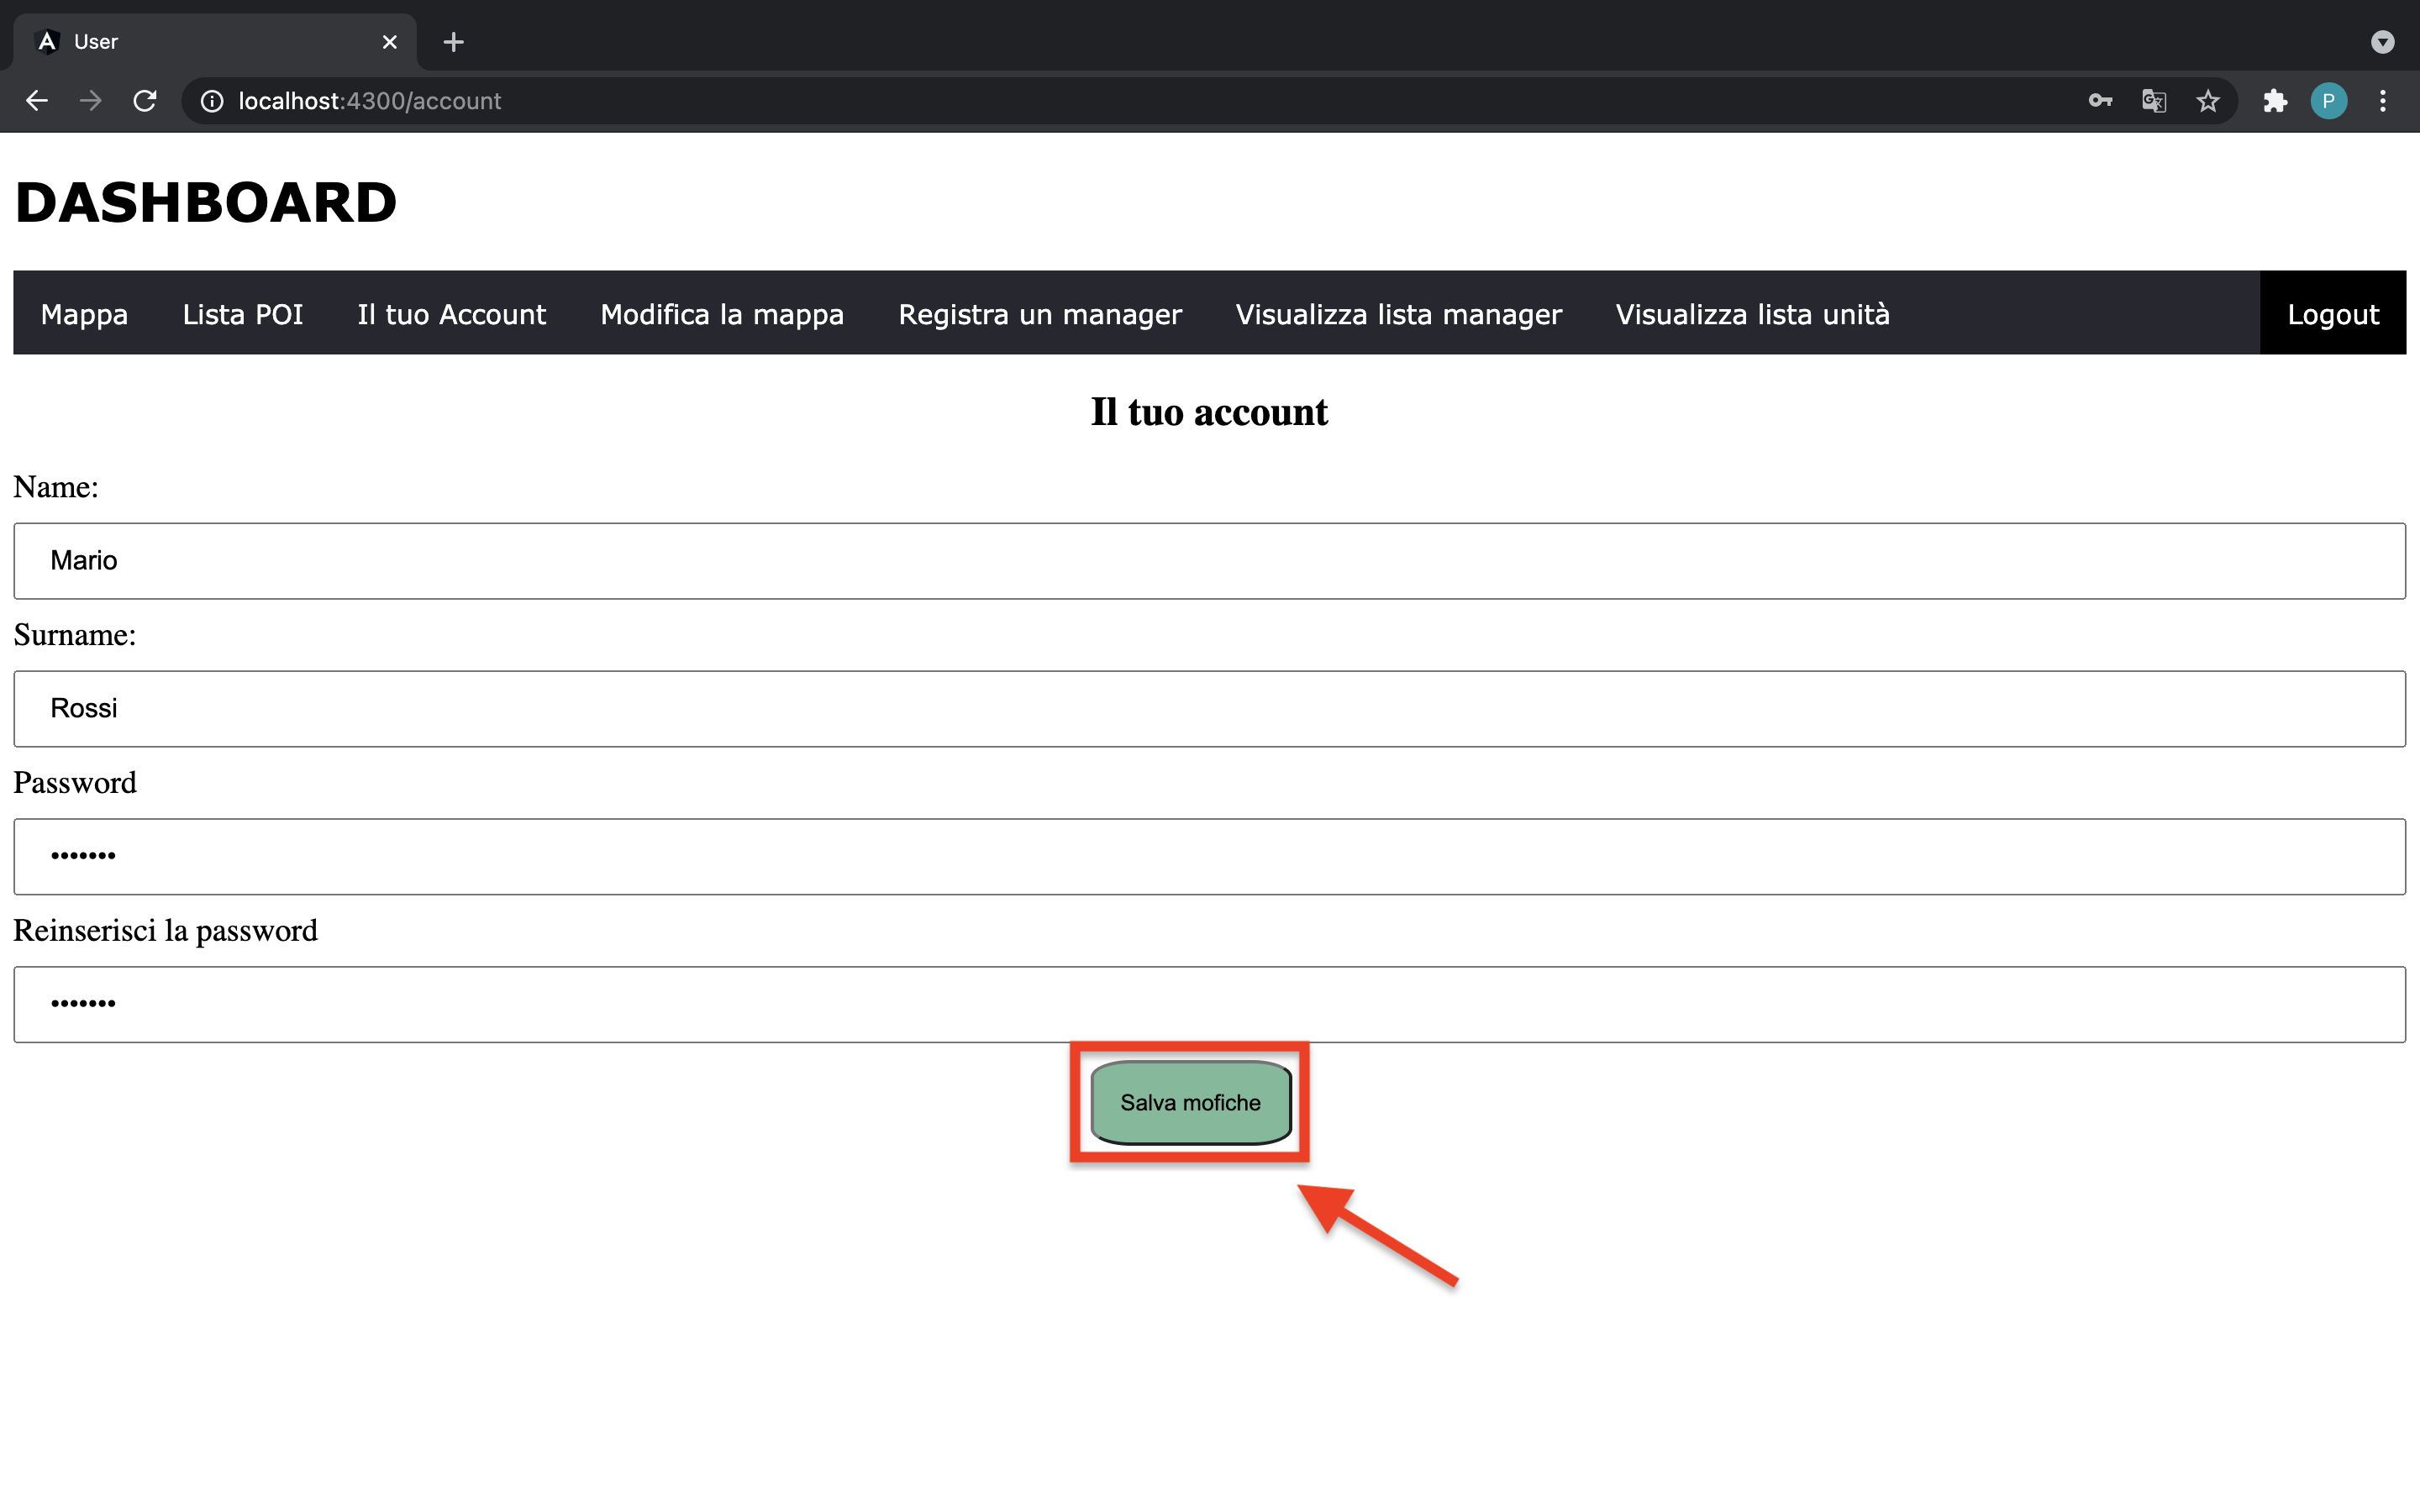
\includegraphics[scale=0.12]{res/images/account_user.png}
    \caption{Schermata proprio profilo}
\end{figure}

\subsection{Registrazione di un nuovo utente}
\begin{itemize}
    \item Dopo l'autenticazione, tramite il menù selezionare il pulsante "Registra un manager";
    \item si viene indirizzati alla pagina con i campi da compilare: Nome, Cognome;
\end{itemize}
\begin{figure}[H]
    \centering
    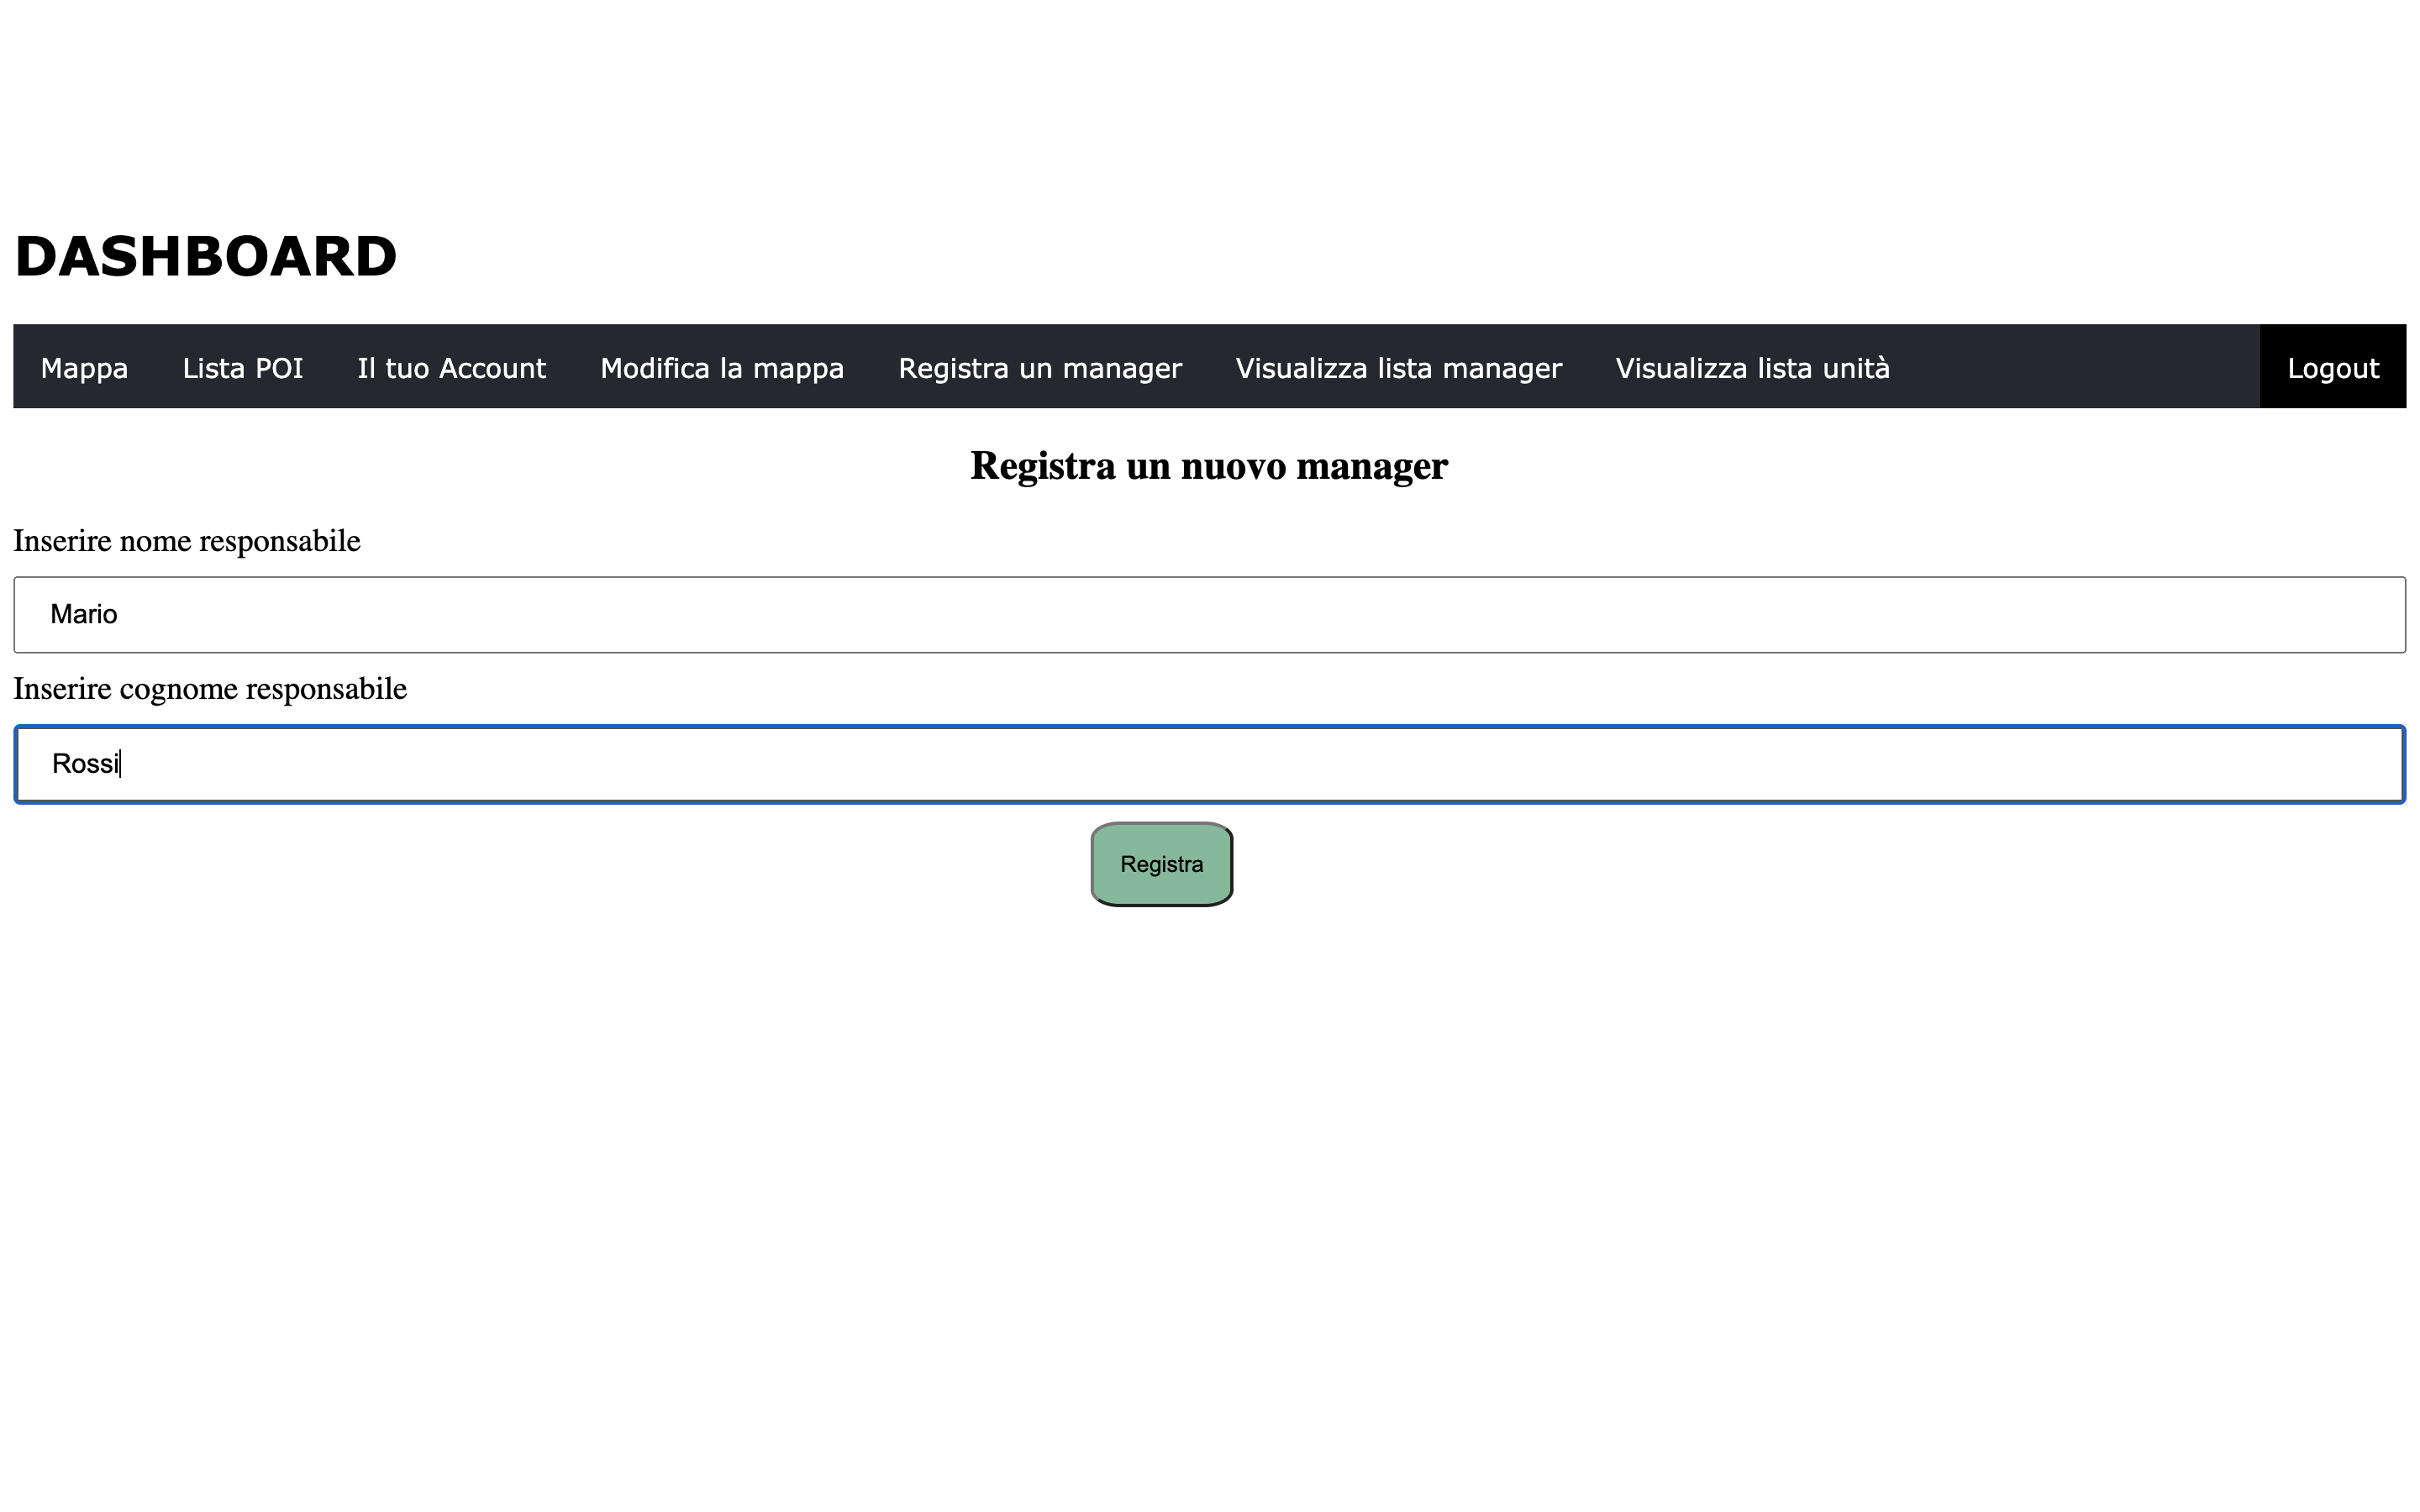
\includegraphics[scale=0.12]{res/images/newmanager_admin.png}
    \caption{Schermata registrazione manager 1}
\end{figure}
\begin{itemize}
    \item inserire i dati e premere sul pulsante "Conferma";
    \item viene visualizzato a video la password e il codice identificativo da riferire al nuovo utente per il suo primo accesso.
\end{itemize}


\begin{figure}[H]
    \centering
    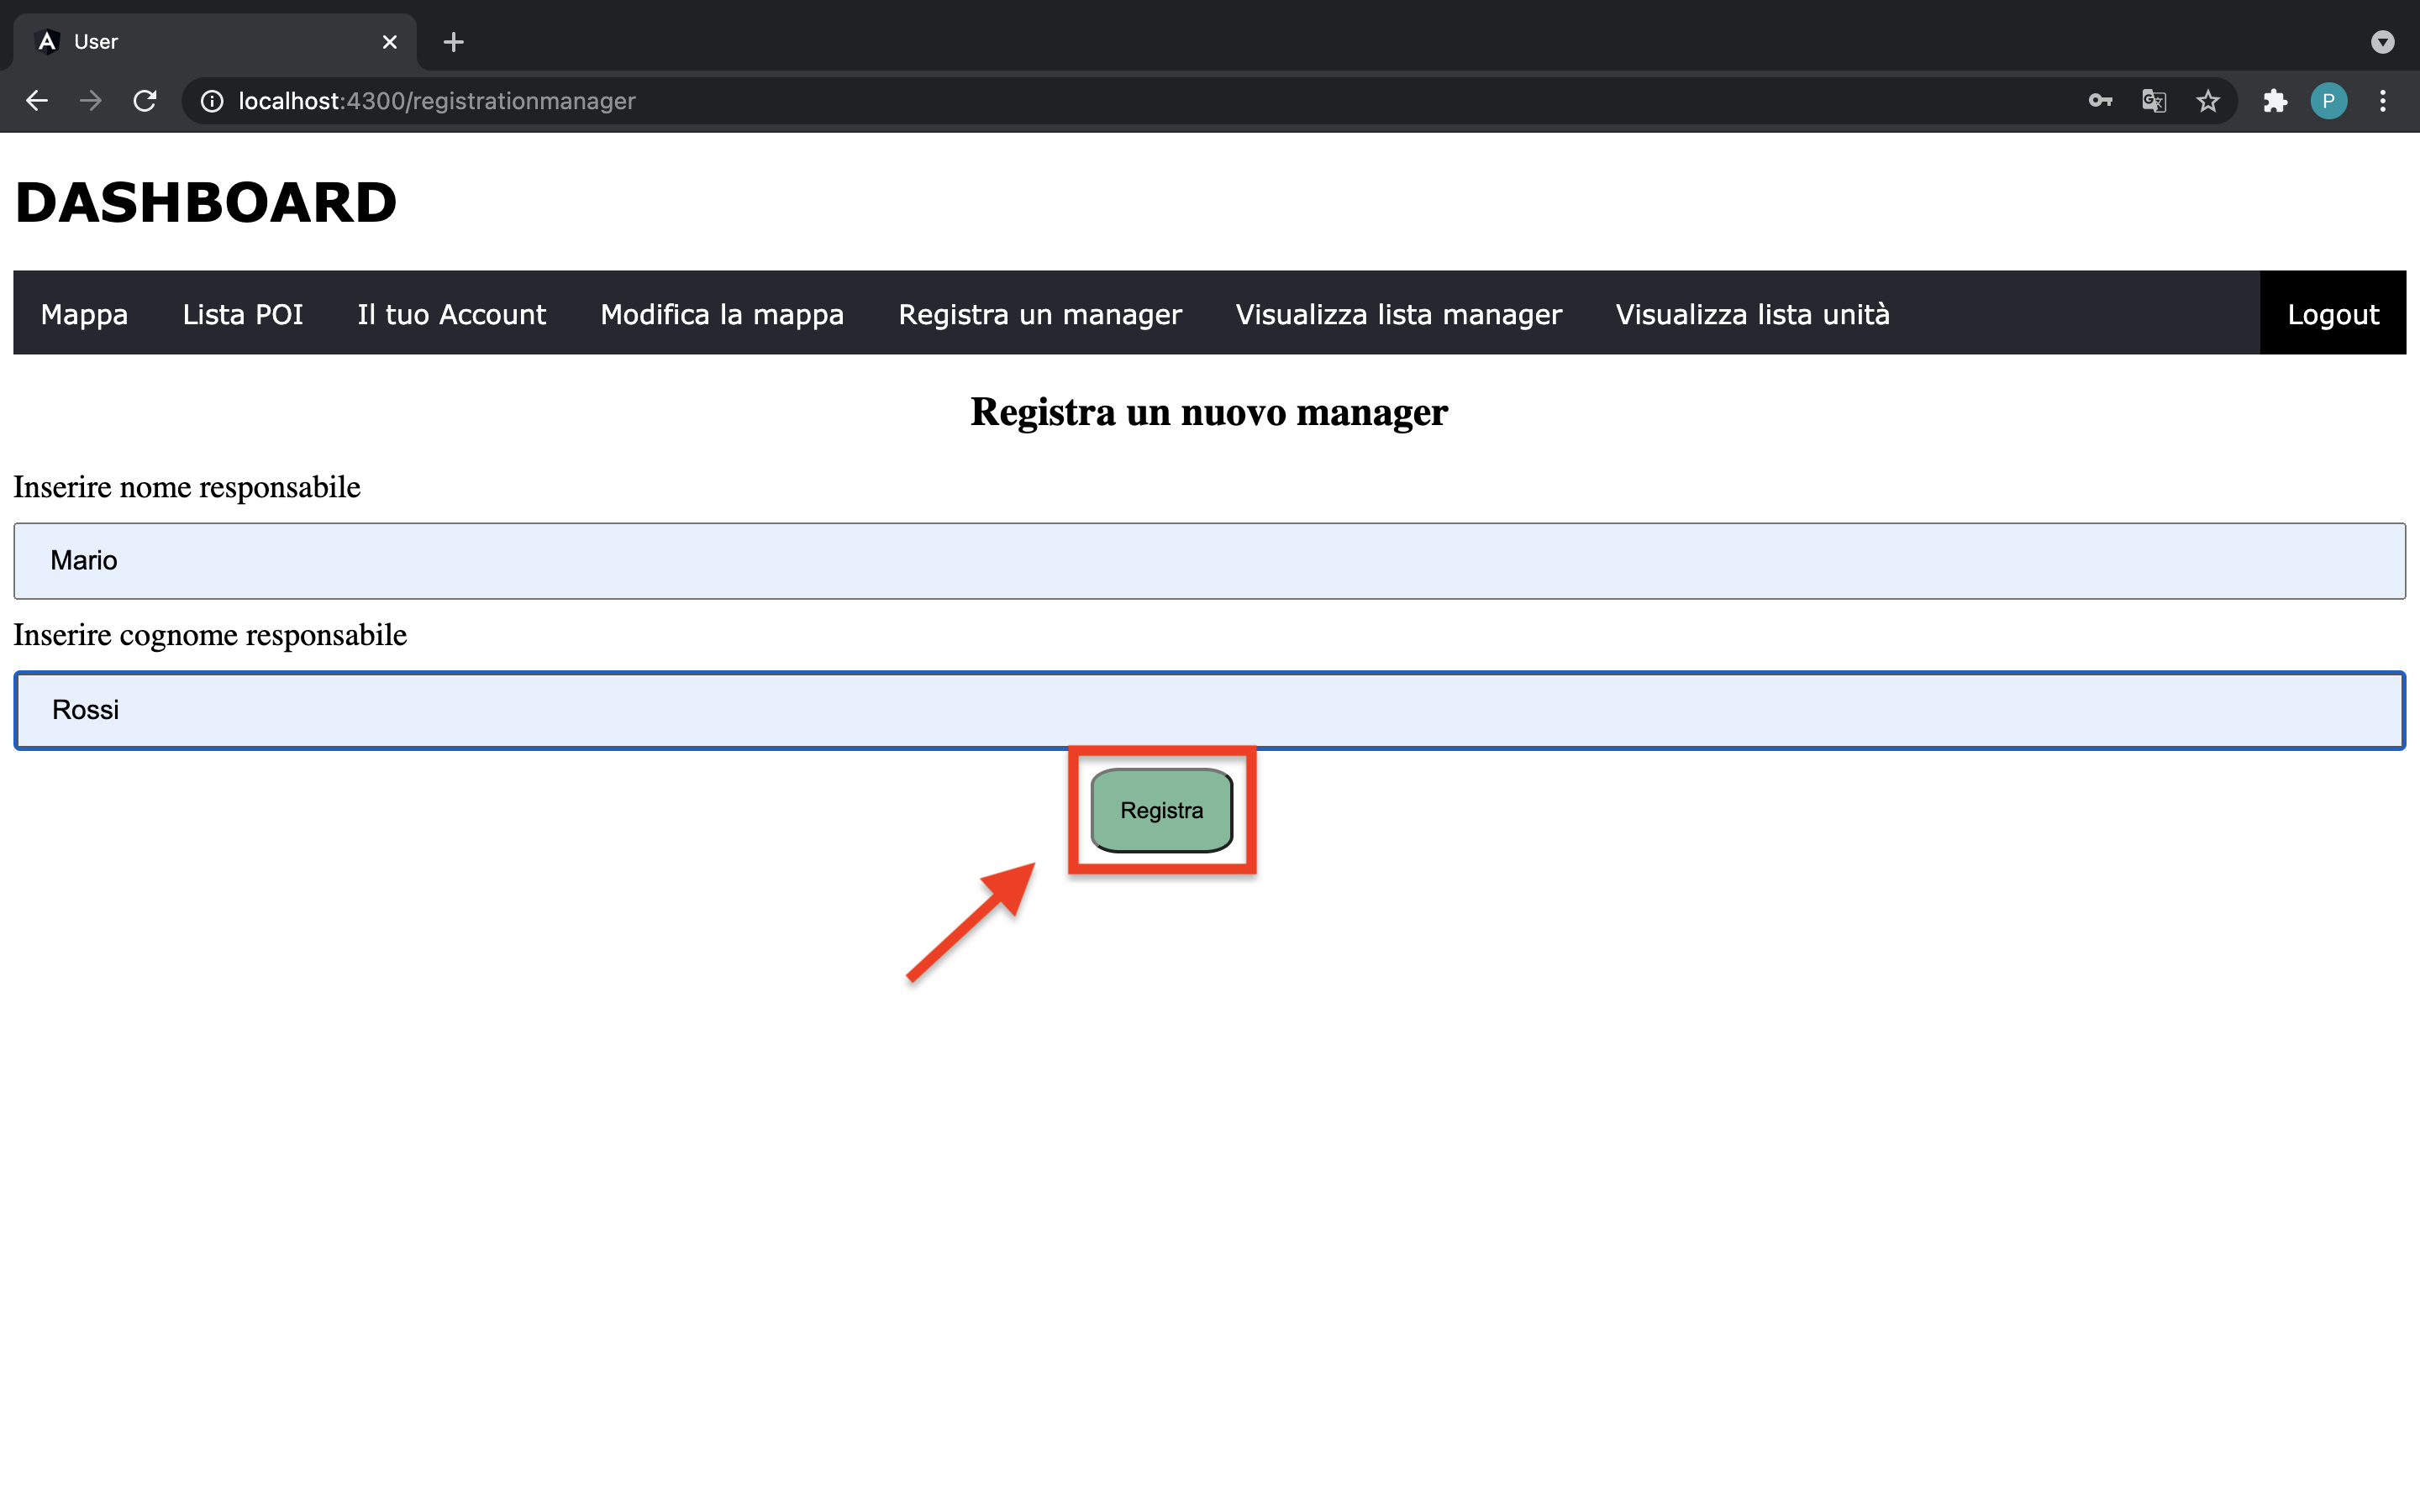
\includegraphics[scale=0.12]{res/images/newmanager_2.png}
    \caption{Schermata registrazione manager 2}
\end{figure}

\subsection{Gestione account già presenti}
\begin{itemize}
    \item Dopo l'autenticazione, tramite il menù selezionare il pulsante "Visualizza lista manager";
    \item si viene indirizzati alla pagina con la lista di tutti gli account presenti;
    \item per ogni account è possibile:
        \begin{itemize}
            \item cambiare i campi "Name" e "Surname" e premere su "Conferma Modifica" per confermare le modifiche;
            \item premere il pulsate "Elimina" per cancellare definitivamente un account dal sistema;
            \item premere il pulsante "Reset password" per cambiare la password di un utente in caso di smarrimento; verrà visualizzata a video la nuova password.
        \end{itemize}
\end{itemize}

\begin{figure}[H]
    \centering
    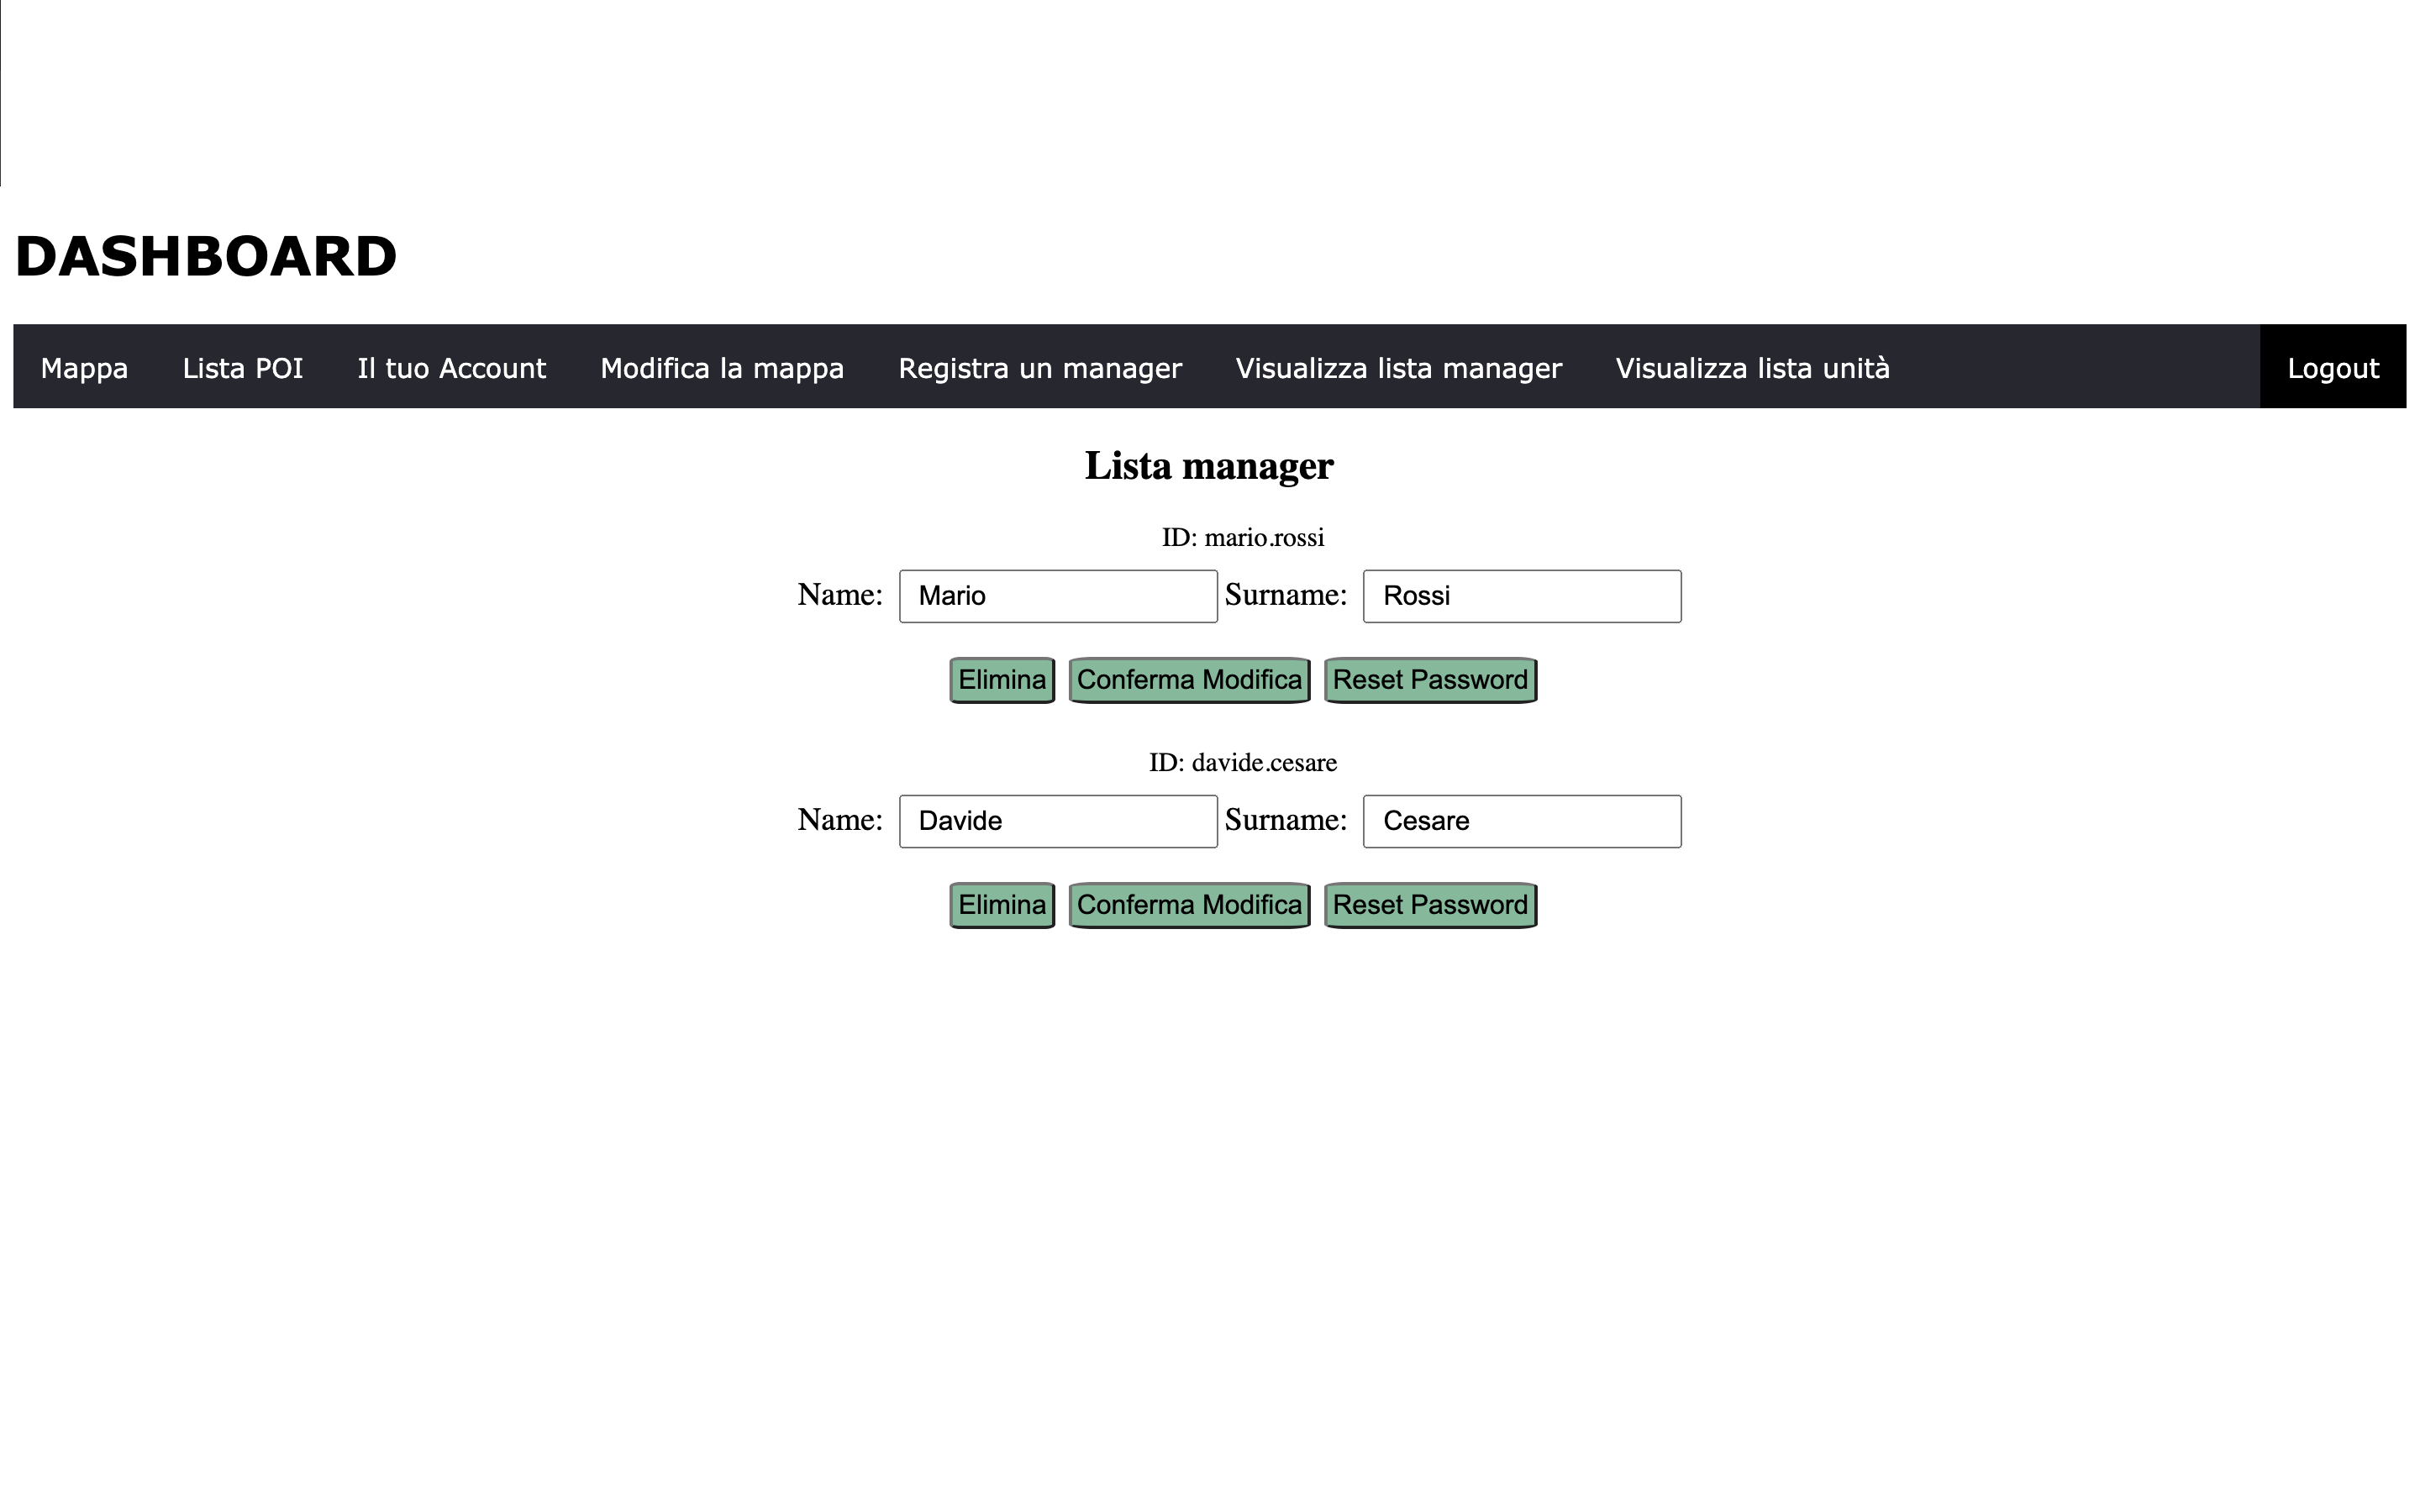
\includegraphics[scale=0.12]{res/images/listmanager_admin.png}
    \caption{Schermata visualizzazione lista di manager}
\end{figure}

\subsection{Modifica mappa del magazzino}
\begin{itemize}
    \item Dopo l'autenticazione, tramite il menù selezionare il pulsante "Modifica mappa";
    \item si viene indirizzati alla pagina con la rappresentazione della mappa;
    \item è possibile intraprendere le seguenti operazioni:
        \begin{itemize}
            \item aggiungere una riga: \\premere sul pulsante "Aggiungi riga" per ampliare la planimetria di una riga;
            \item eliminare una riga: \\premere sul pulsante "Rimuovi riga" per diminuire la planimetria di una riga;
            \item aggiungere una colonna: \\premere sul pulsante "Aggiungi colonna" per ampliare la planimetria di una colonna;
            \item eliminare una colonna: \\premere sul pulsante "Rimuovi colonna" per diminuire la planimetria di una colonna;
            \begin{figure}[H]
                \centering
                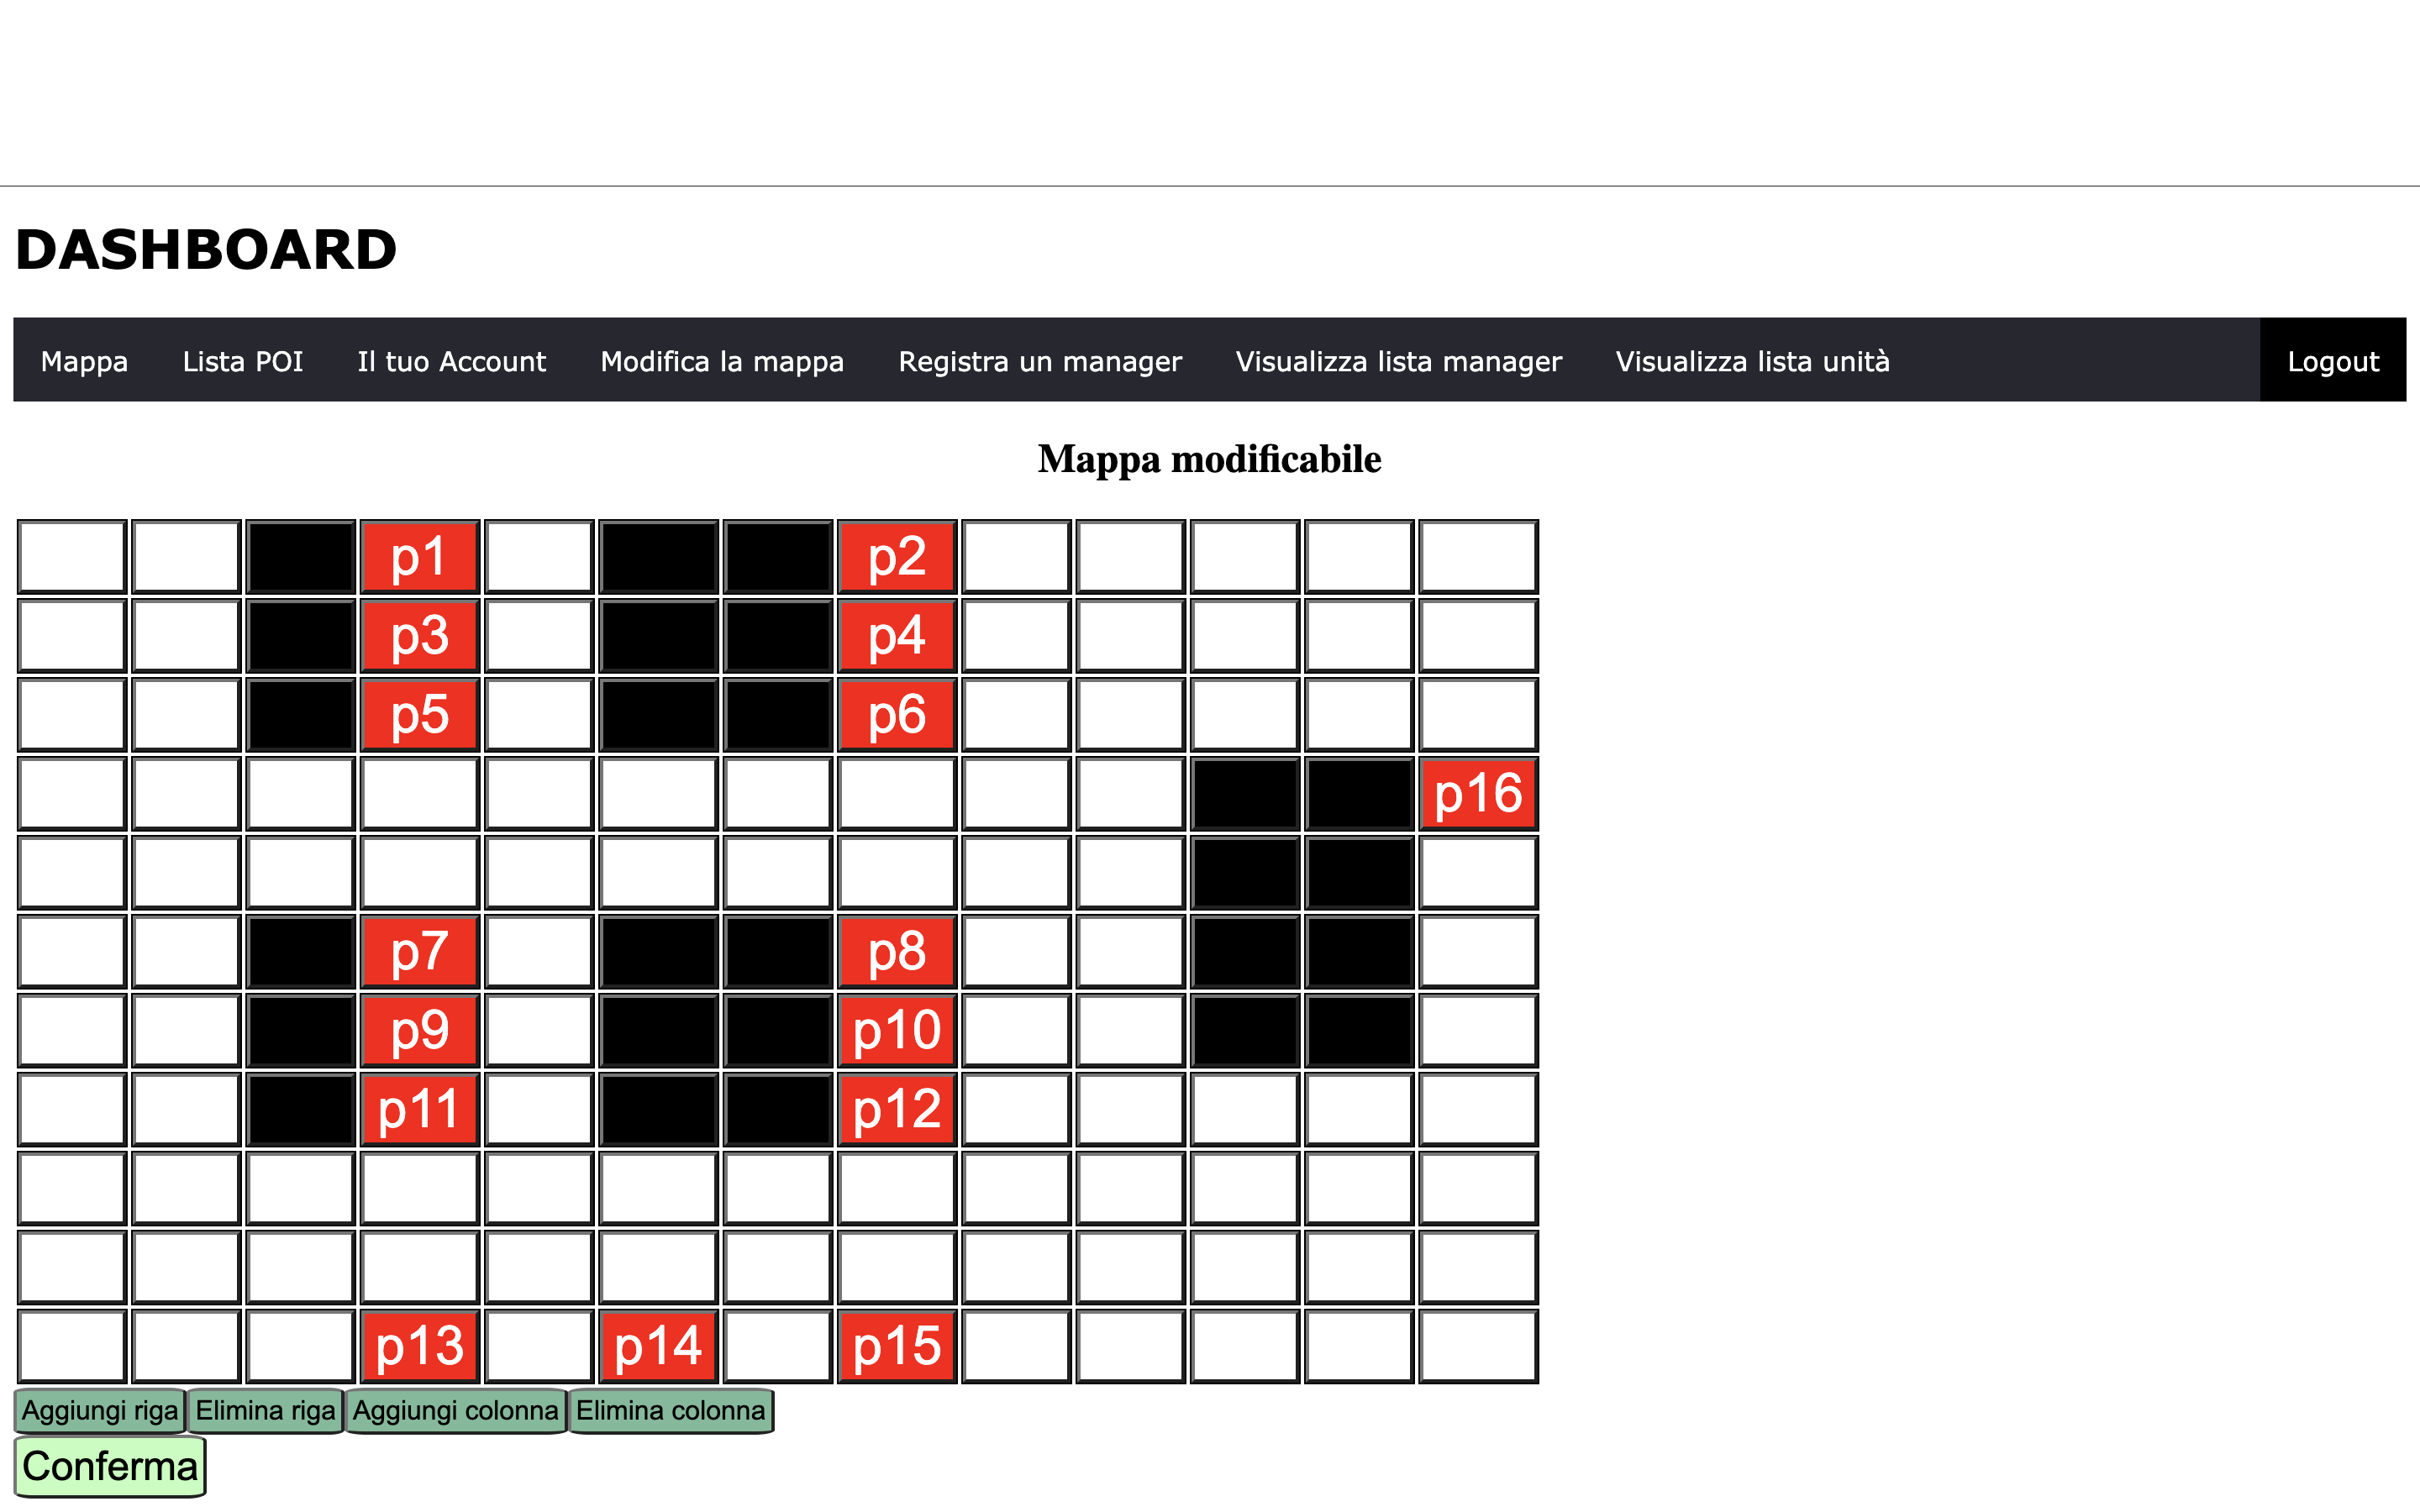
\includegraphics[scale=0.12]{res/images/managemap_admni1.png}
                \caption{Schermata modifica mappa}
            \end{figure}
            \item cambiare il tipo di cella: \\premere sulla cella nella mappa che si intende modificare. Verrà allora visualizzata un'interfaccia con i colori possibili (bianco: zona transitabile, nero: zona non transitabile, frecce: sensi unici, rosso: POI). Nel caso di POI è possibile scrivere l'identificativo. \\Una volta scelto premere sul tasto "Conferma".
        \end{itemize}
        \begin{figure}[H]
            \centering
            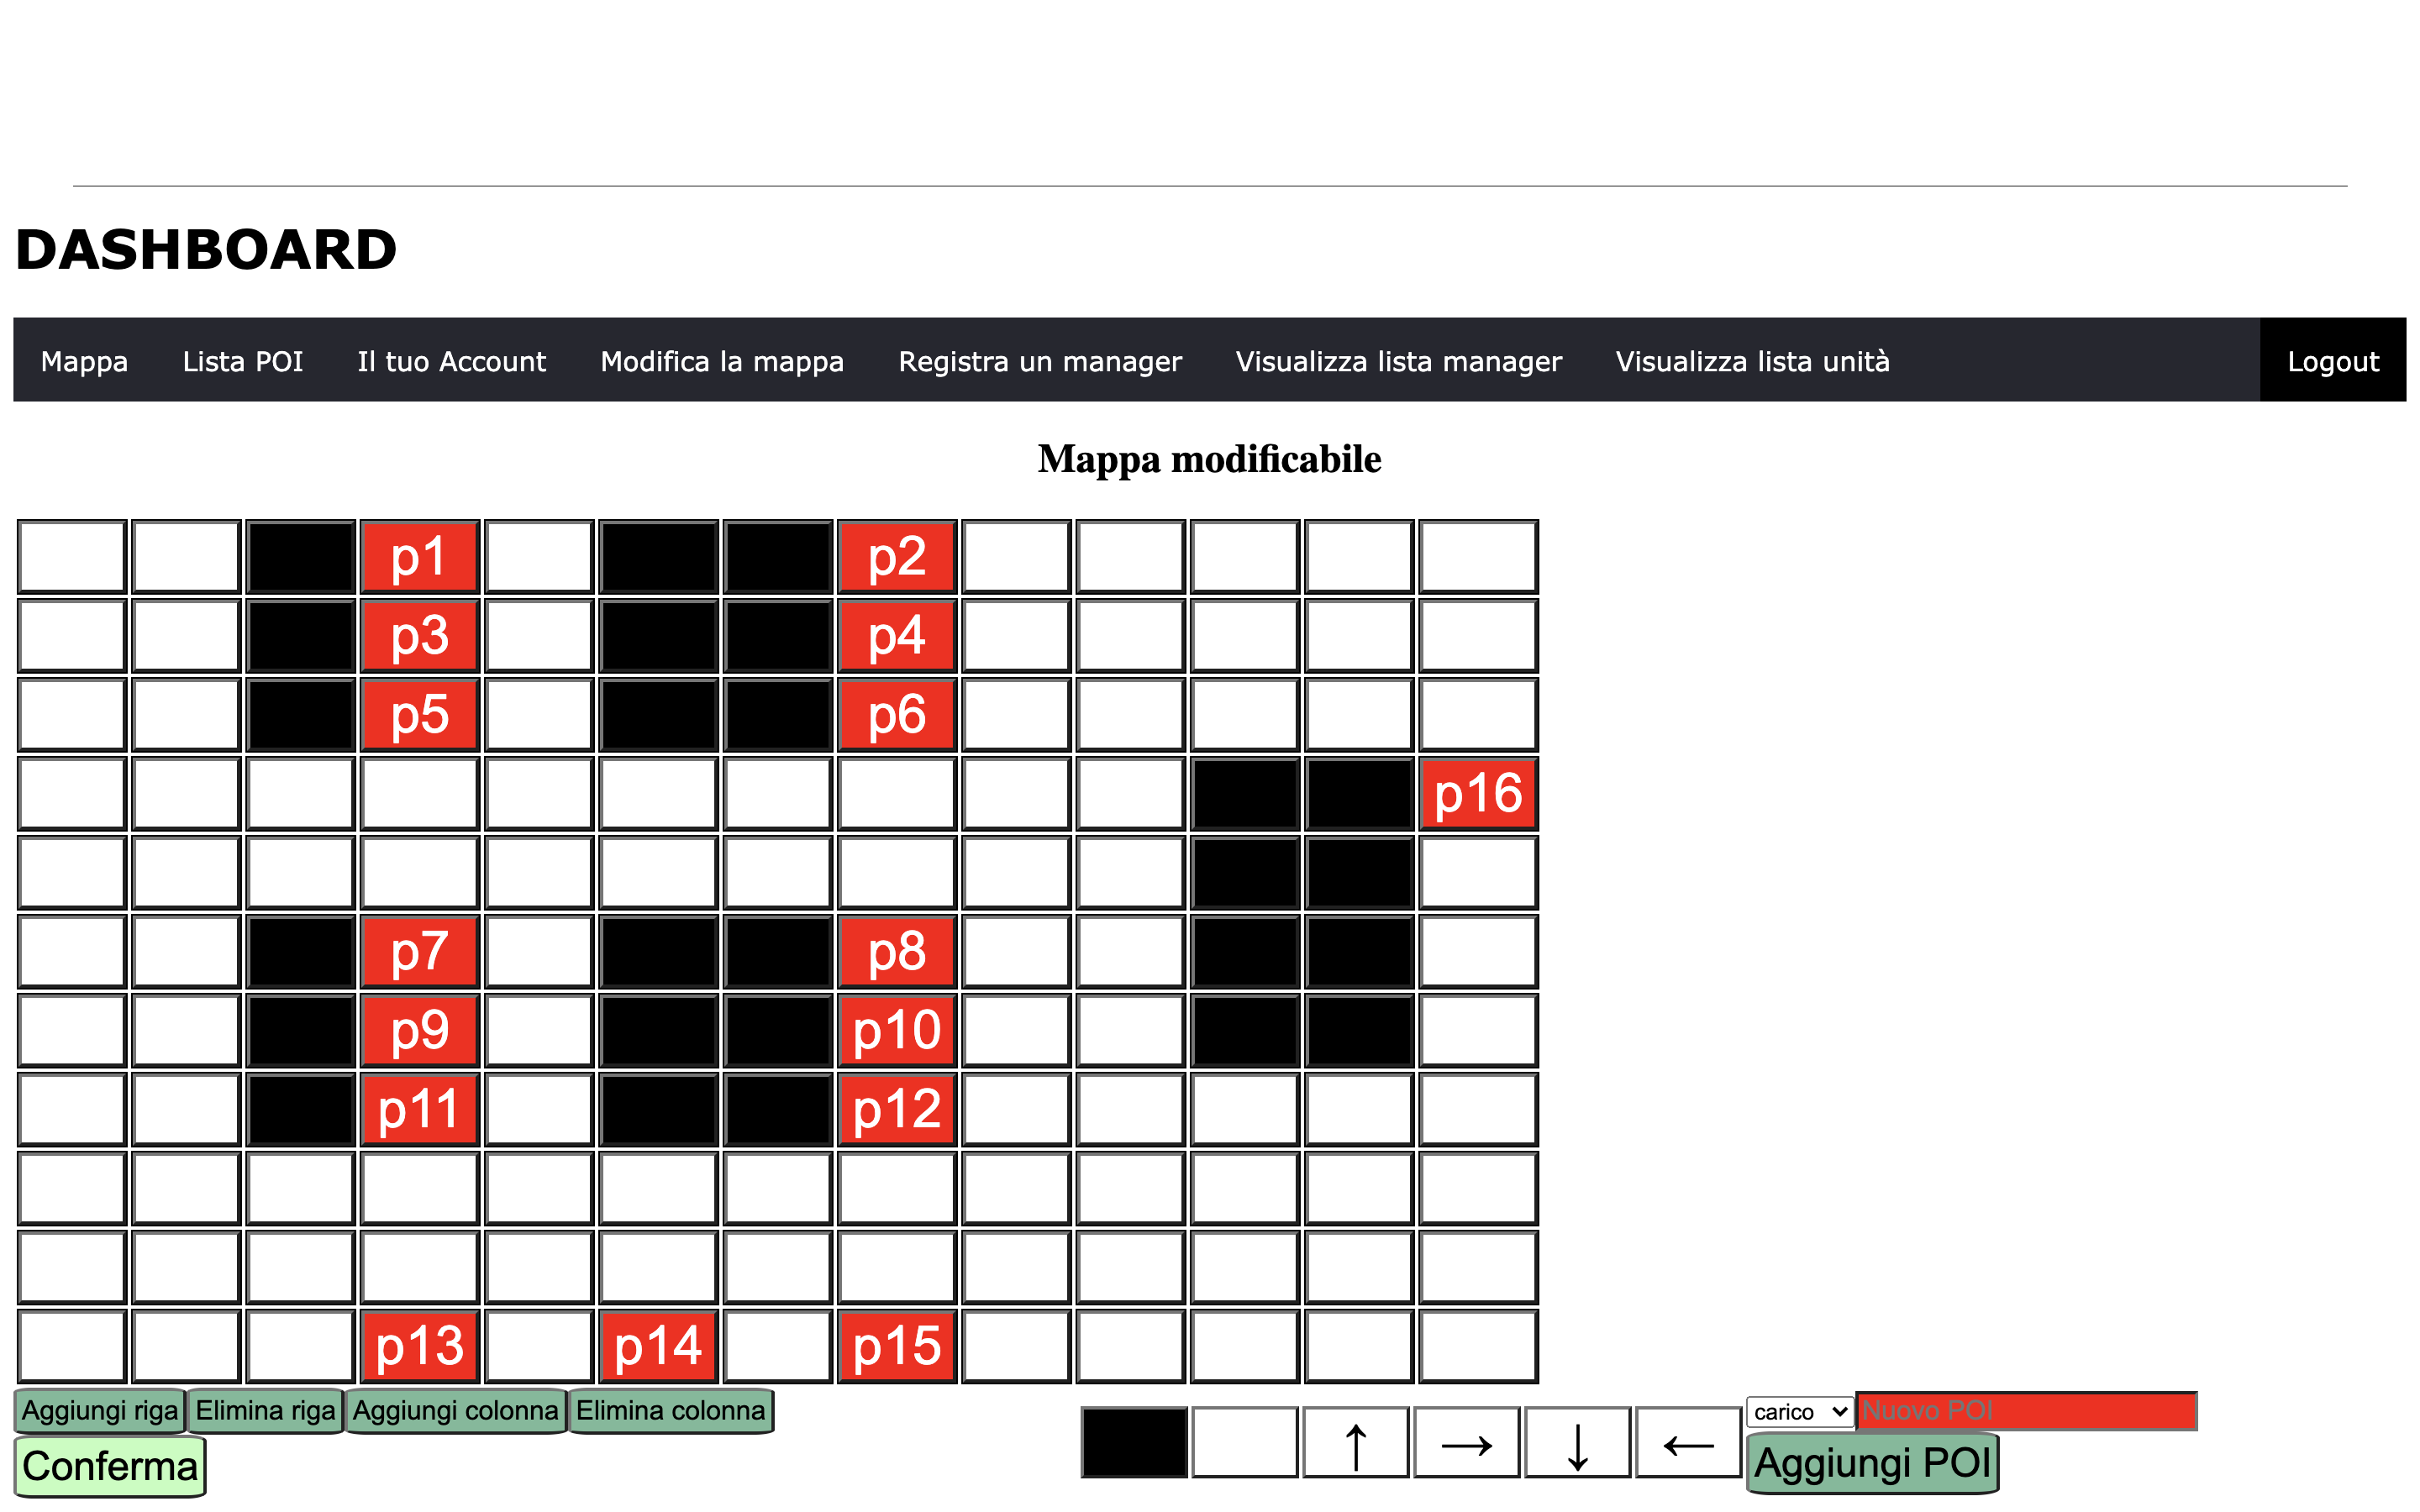
\includegraphics[scale=0.12]{res/images/managemap2.png}
            \caption{Schermata modifica mappa}
        \end{figure}
    \item quando si è soddisfatti delle modifiche premere sul pulsante "Conferma".
\end{itemize}

\begin{figure}[H]
    \centering
    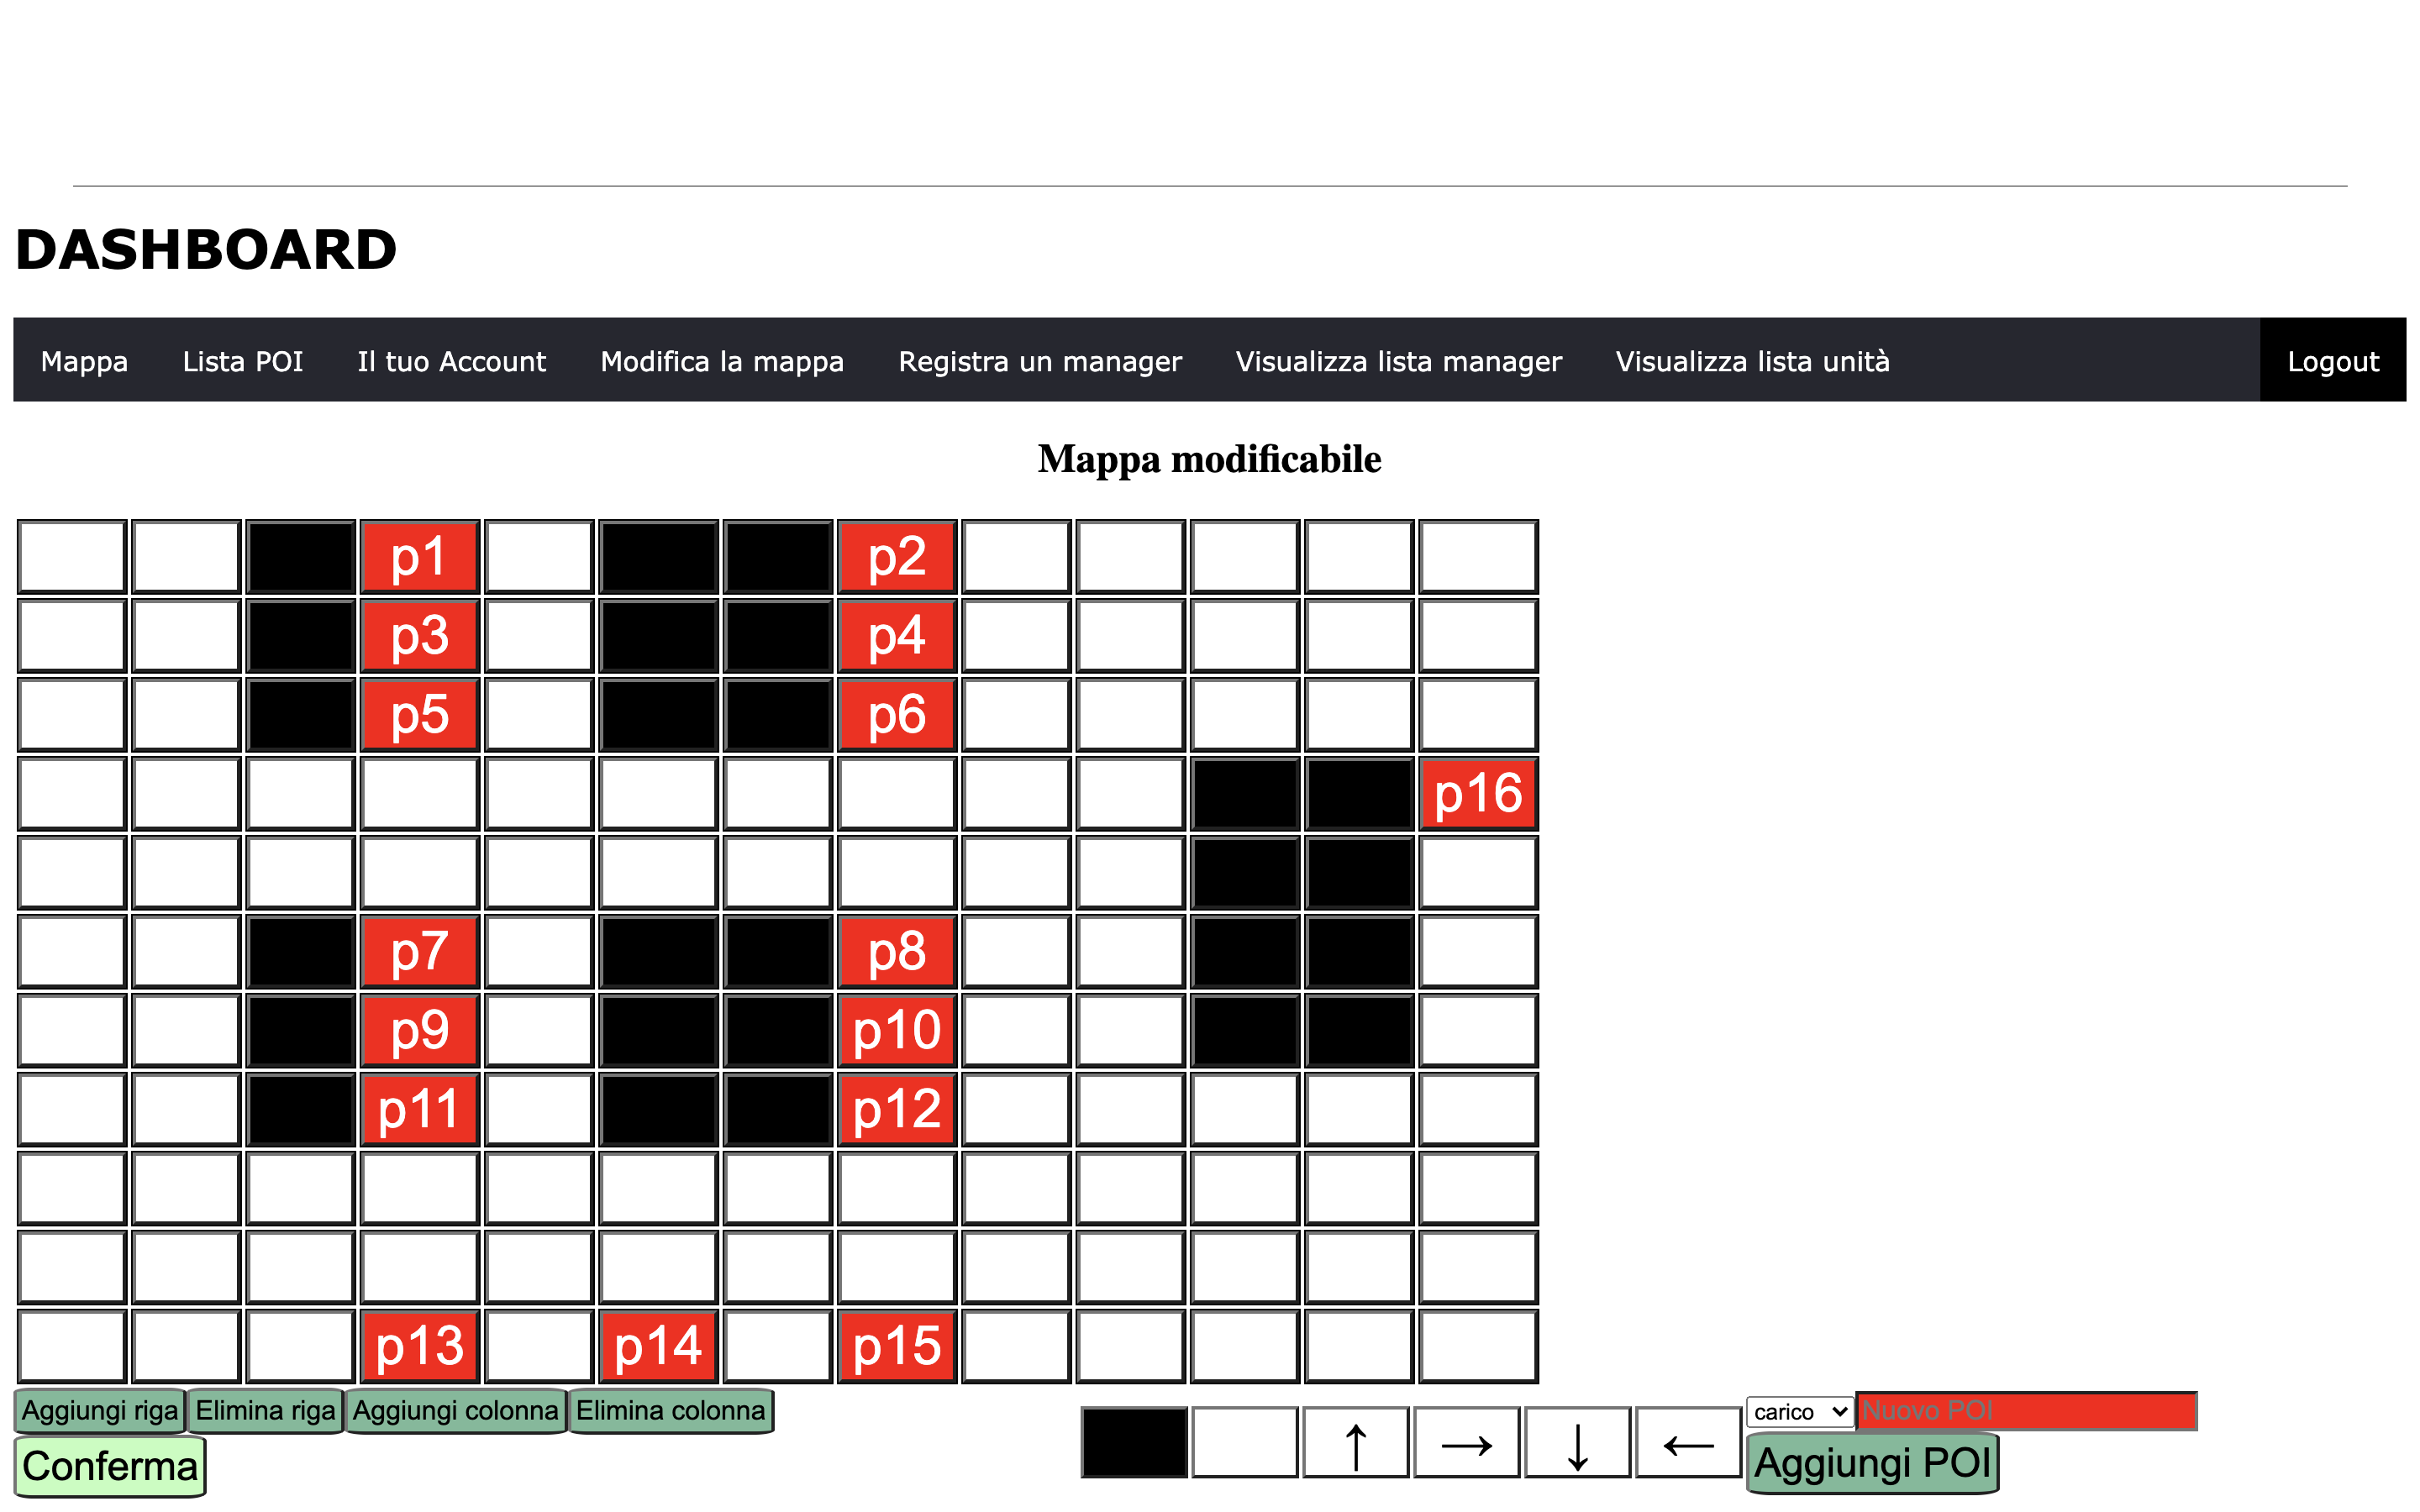
\includegraphics[scale=0.12]{res/images/managemap2.png}
    \caption{Schermata guida automatica dell'unità}
\end{figure}

\subsection{Gestione unità}
\begin{itemize}
\item Dopo l'autenticazione, tramite il menù selezionare il pulsante "Visualizza lista unità"; è possibile effettuare le seguenti operazioni:
    \item aggiungere una nuova unità: \\inserire il codice identificativo nel form e premere il pulsante "Registra";
    \item eliminare un'unità presente: 
    \begin{itemize}
        \item selezione dal menu a tendina l'id dell'untià che si intende eliminare;
        \item premere sul pulsante "Elimina" per confermare l'eliminazione.
    \end{itemize}
\end{itemize}
\begin{figure}[H]
    \centering
    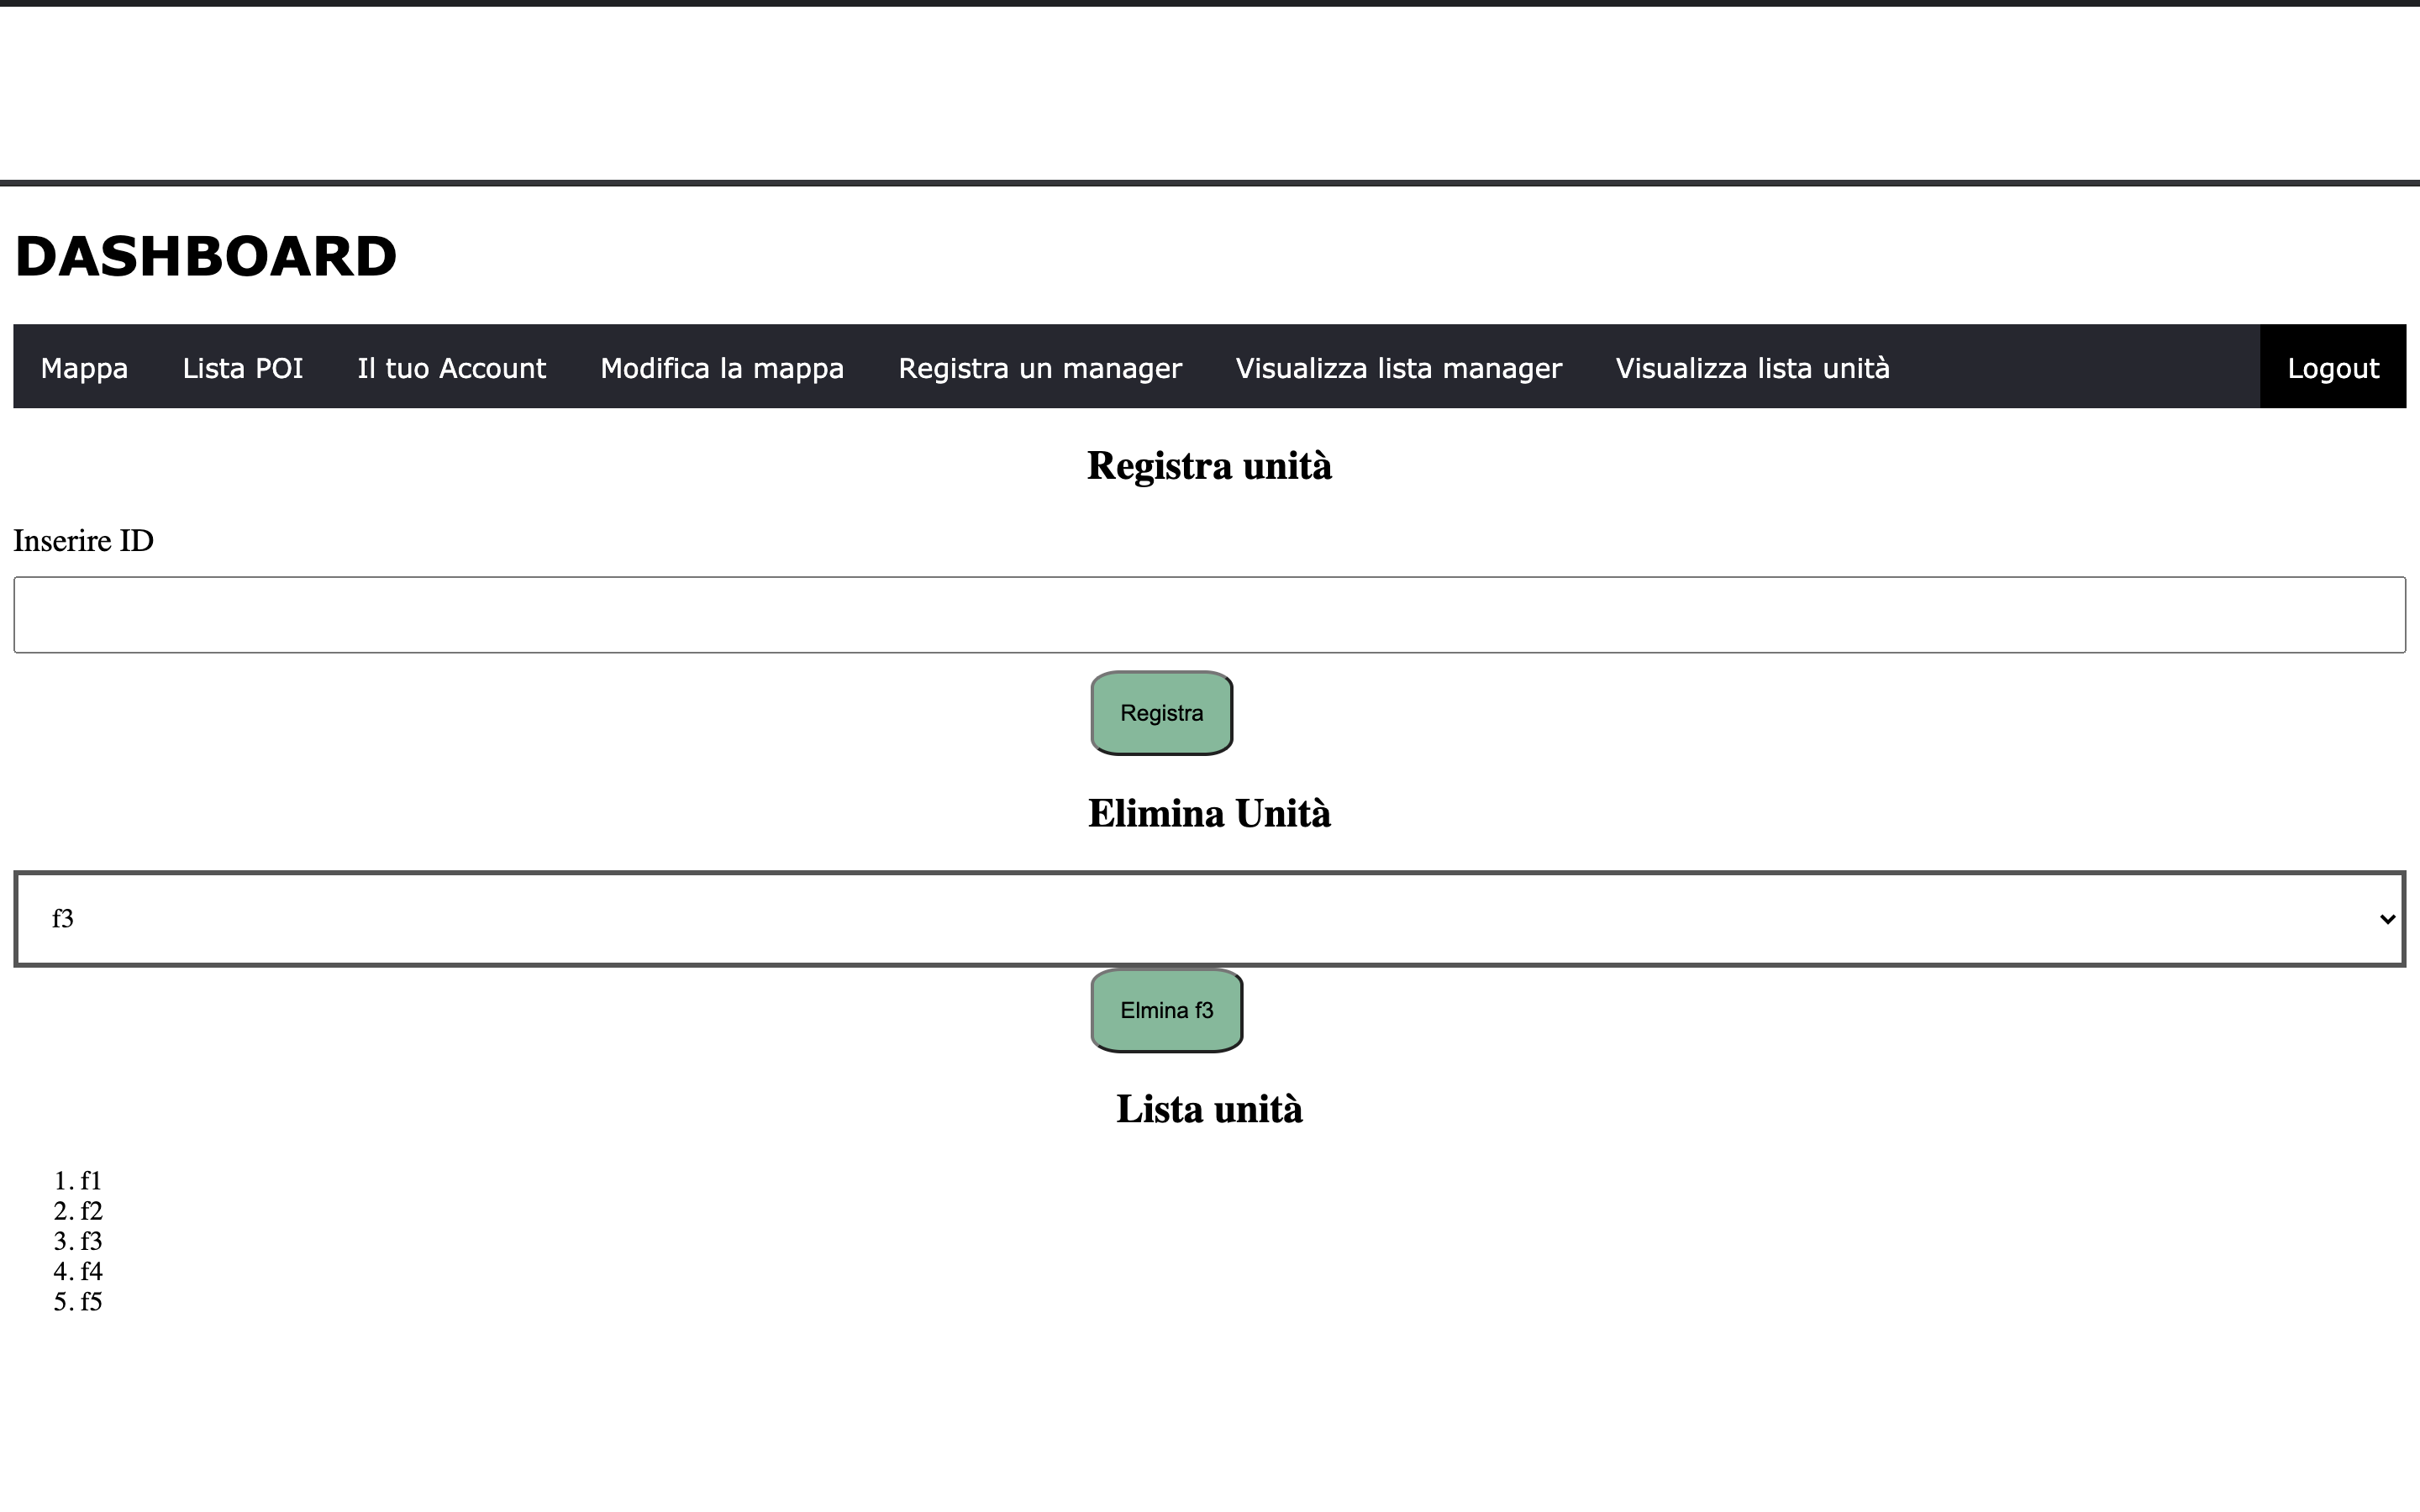
\includegraphics[scale=0.12]{res/images/newunit_admin.png}
    \caption{Schermata lista unità}
\end{figure}